\documentclass[a4paper, 11pt,oneside,openany, danish]{memoir} % Starter dokumentet af klassen memoir


%%%%%%%%%%%%%%%%%%%%%%%
		       % PREAMBLE %			
%%%%%%%%%%%%%%%%%%%%%%%



% Papirstørrelse og margener
\usepackage[paper=a4paper, hmargin=1.1in, vmargin=1.1in]{geometry}

% Font encoding og sprog
\usepackage[T1]{fontenc}				% Output encoding
\usepackage[utf8]{inputenc}				% Input encoding
\usepackage[danish]{babel}				% Sprog (orddeling)
\renewcommand{\danishhyphenmins}{22} 	% bedre orddeling, minimum to tegn før og efter deling
\usepackage{lmodern}  					% gør underscores pænere
\usepackage{microtype} 					% laver micro ændringer i text for at udgå luft og orddeling


%% Forside text
%\usepackage{soul} % lege lege
%\sodef\an{}{0.2em}{.9em plus.6em}{1em plus.1em minus.1em}
%\newcommand\stext[1]{\an{\scshape#1}}

% Fyldetekst (Lorem ipsum)
\usepackage{blindtext}

% Til kodeeksempler
\usepackage{listings}

\lstdefinestyle{customc}{
	belowcaptionskip=1\baselineskip,
	breaklines=true,
	frame=L,
	xleftmargin=\parindent,
	language=C,
	showstringspaces=false,
	basicstyle=\footnotesize\ttfamily,
	keywordstyle=\bfseries\color{green!40!black},
	commentstyle=\itshape\color{purple!40!black},
	identifierstyle=\color{blue},
	stringstyle=\color{orange},
}

\lstdefinestyle{customasm}{
	belowcaptionskip=1\baselineskip,
	frame=L,
	xleftmargin=\parindent,
	language=[x86masm]Assembler,
	basicstyle=\footnotesize\ttfamily,
	commentstyle=\itshape\color{purple!40!black},
}

\lstset{escapechar=@,style=customc}

% Tabeller
\usepackage{booktabs}
\usepackage{threeparttable}
\usepackage[tableposition=top]{caption}
\usepackage{tabularx}
\usepackage{multirow}					% For at lave pæne tabeller
\usepackage{hhline}						% For at lave endnu pænere tabller
\newcolumntype{C}{>{\let\newline\\\arraybackslash\hspace{0pt}}X}
\usepackage{float}
%matematik
\usepackage{amsmath,amssymb,mathtools,bm}
\newcommand{\tsub}[1]{_{\textup{#1}}}
\def\doubleunderline#1{\underline{\underline{#1}}}
\usepackage[separate-uncertainty = true,multi-part-units=single]{siunitx}
\usepackage{longtable}

% XColor: Farver
\usepackage[svgnames,dvipsnames,x11names]{xcolor}

% Figurer og floats
\usepackage[]{graphicx}
\graphicspath{{figurer/}}
\usepackage{placeins}
\usepackage{float}			% Muliggoer eksakt placering af floats, f.eks. \begin{figure}[H]

%%% Tegning af kasser
%\usepackage{calc,graphicx,color}
%\definecolor{mygreen}{rgb}{0,0.6,0}
%\definecolor{mygray}{rgb}{0.5,0.5,0.5}

% Biblatex til referencer
\usepackage[backend=bibtex]{biblatex}
\addbibresource{bibfil.bib}





% Hyper ref
\usepackage[ unicode=true, colorlinks=false, linktocpage=true, 
pdfborder={0 0 0}, pdfstartpage=1, pdfstartview=FitV, breaklinks=true,
pdfpagemode=UseNone, pageanchor=true, pdfpagemode=UseOutlines,
plainpages=false, bookmarksnumbered, bookmarksopen=true,
bookmarksopenlevel=1, hypertexnames=true, pdfhighlight=/O, urlcolor=Black,
linkcolor=Black, citecolor=Black]{hyperref}

% Clever ref
\usepackage{cleveref}



\settocdepth{subsection}
\setsecnumdepth{subsection}

% Sidetal
% Sidetal
\let\footruleskip\undefined
\usepackage{fancyhdr}
\usepackage{lastpage}
\pagestyle{fancy} 
\fancyhf{} 

\fancyhead[R]{\leftmark}
\fancyfoot[R]{\thepage \hspace{0.008in} af \pageref{LastPage}}

\fancypagestyle{}{
	\renewcommand{\headrulewidth}{0pt}
	\fancyhf{}
	\fancyfoot[R]{\thepage \hspace{0.008in} af \pageref{LastPage}}%
	
}


% Starten på dokumentet
\begin{document}


%%%%%%%%%%%%%%%%%%%%%%%
		       % FORSIDEN %			
%%%%%%%%%%%%%%%%%%%%%%%

% !TEX root = ../prj4projektdokumentation.tex
% SKAL STÅ I TOPPEN AF ALLE FILER FOR AT MASTER-filen KOMPILERES 
\thispagestyle{empty}
{\centering
	{\scshape\LARGE Aarhus Universitet \par}
	\vspace{1cm}
	{\scshape\Large 4. semesterprojekt gruppe 1\par}
	{\scshape\Large Projektdokumentation\par}
	\vspace{1.5cm}
	{\huge\bfseries Spændingsregulator\par}
	\vspace{2cm}
	{\Large
		201509249 - Caroline Møller Sørensen\\
		201611140 - Sophia Amailie Mortensen\\
		201505195 - Dennis Slot Larsen \\
		201505115 - Laurids Givskov Jørgensen\\
		201508333 - Søren Jensen\\
		13114 - Jeppe Hansen\\  }
	\vfill
	Vejleder\par
	Emir Pasic
	
	\vfill
	
	{\large \today\par}
	\par}




\frontmatter
%%%%%%%%%%%%%%%%%%%%%%%
             % RESUME & ABSTRACT %			
%%%%%%%%%%%%%%%%%%%%%%%



%%%%%%%%%%%%%%%%%%%%%%%
         % INDHOLDSFORTEGNELSE %			
%%%%%%%%%%%%%%%%%%%%%%%

\tableofcontents

%%%%%%%%%%%%%%%%%%%%%%%
                        % KAPITLER %			
%%%%%%%%%%%%%%%%%%%%%%%

\mainmatter
% !TEX root = ../prj4projektdokumentation.tex
% SKAL STÅ I TOPPEN AF ALLE FILER FOR AT MASTER-filen KOMPILERES 

\chapter{Introduktion}

\section{Problemformulering}
Når belastningerne i et distributionssystem ændres, vil spændingsniveauet variere. Det er vigtigt, at spændingsniveauet holdes stabilt. Hvordan sikres dette?
% !TEX root = ../prj4projektdokumentation.tex
% SKAL STÅ I TOPPEN AF ALLE FILER FOR AT MASTER-filen KOMPILERES 

\chapter{Projektbeskrivelse}

Formålet med dette projekt, er at opbygge et system, der simulerer det danske transmissionssystem. For energileverandører i Danmark er det et lovmæssigt krav, at spændingsforsyningen hos forbrugerne altid ligger på $\pm$ 230 volt, og det ønskes at undersøge mulighederne for at opfylde dette.\\ 
I dette projekt vil fokus være på stykket fra distributionstransformer og ud til forbrugere/belastninger. Systemet skal bestå af en spændingsregulator (trinkobler), en distributionslinje og to eller flere varierende belastninger. Det ønskes at måle strøm, spænding, power factor og effektretning således, at spændingsregulatoren hele tiden kan holde spændingen på $\pm$ et givent niveau, selvom belastningen ændres. Normalt måles disse værdier ved distributionstransformeren, men i dette projekt ønskes det at måle hos hver enkelt belastning. På den måde fås en bedre overvågning af systemet og bedre mulighed for at observere hvilken betydning, f.eks. belastningens afstand til distributionstransformeren har for spændingsniveauet.\\ Systemet skal have to indstillinger – en til manuelt valg af spændingsniveau og en til automatisk valg af passende spændingsniveau.\\ 
Det ønskes desuden at kunne måle frekvensindholdet i systemet for at kunne observere et eventuelt indhold af harmoniske. De harmoniske i systemet er højfrekvente og vil afsætte varme i transformerne og dermed forkorte deres levetid. Det er derfor relevant at kende til indholdet af disse.\\ 
Det er et krav, at målte værdier i systemet vises på en skærm. 

\begin{figure}[htbp] % (alternativt [H])
	\centering
	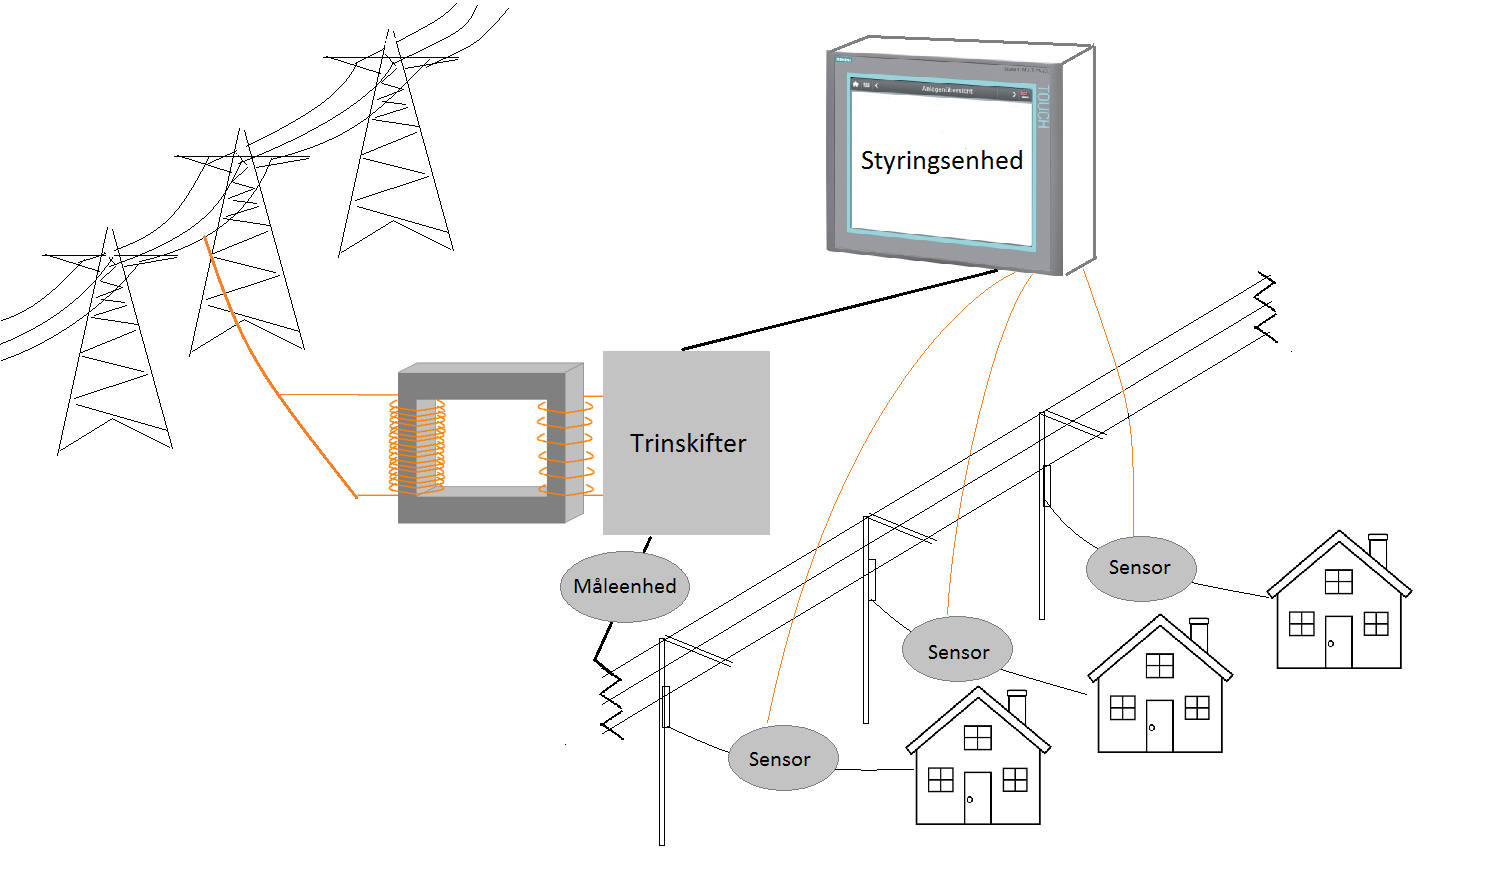
\includegraphics[width=0.7\textwidth]{Figure/RigtBillede}
	\caption{Visuel fremvisning af system}
	\label{fig:Rigtbillede}
\end{figure}
% !TEX root = ../prj4projektdokumentation.tex
% SKAL STÅ I TOPPEN AF ALLE FILER FOR AT MASTER-filen KOMPILERES 


\chapter{Termliste}

\begin{table}[htbp]
	\centering
	\begin{tabular}{|l|l|}
		\hline
		\textbf{Term} 	& \textbf{Beskrivelse} \\\hline
		Spændingsregulator	& Samlet system \\\hline
		Trintransformer	& Transformer med variabelt omsætningsforhold \\\hline
		Trinskifter	& Omfatter trintransformer og relækredsløb  \\\hline
		Styringsenhed	& PLC, HMI og Arduino \\\hline
		Centralt	& Ved trinskifter \\\hline
		Decentralt 	& Ved forbrugeren \\\hline
		Måleenhed	& PSoC og tilhørende hardware \\\hline
		
	\end{tabular}
	\caption{Termbeskrivelse}
	\label{tab:termbeskrivelsen}
	
\end{table}
% !TEX root = ../prj4projektdokumentation.tex
% SKAL STÅ I TOPPEN AF ALLE FILER FOR AT MASTER-filen KOMPILERES 
\chapter{Kravspecifikation}
% !TEX root = ../../prj4projektdokumentation.tex
% SKAL STÅ I TOPPEN AF ALLE FILER FOR AT MASTER-filen KOMPILERES 

\section{Systembeskrivelse}

Systemet der er udviklet har til opgave at regulere spændingsniveauet på en distributionslinje, afhængigt af målingerne fra sensorer ved hver forbruger.
I dette projekt er det ikke muligt at realisere, derfor udvikles et produkt, der kan simulere scenariet. Det simuleres ved at skalere spændingsniveauet fra standardniveauet på 230V ned til 4V på distributionssiden. Dette gør det muligt at arbejde med en 8-trins transformer med specifikationen 24V/8-0V.\\
I prototypen er udviklet en impedans til simulering af en distributionslinje med en længde svarende til en typisk distributionslinje.\\
På distributionslinjen er så placeret et antal belastninger, der skal illustrere en husstand. Disse er designet således, at skalering passer med resten af systemet. Dette er rammen systemet skal arbejde indenfor. \\
To typer måleenheder er fremstillet; en placeret centralt på sekundær side af transformeren, og en som er placeret ved hver belastning. De decentrale måleenheder kan måle spænding, strøm og faseforskydning. Den centrale måleenhed kan også måle indeholdet af harmoniske frekvenser. Systemets frekvens er 50Hz ligesom frekvensen på det danske elnet.\\
Data fra måleenhederne samles så i en styringsenhed, der har til opgave at regulere spændingsniveauet, så det altid ligger på 4V på distributionssiden ved at skifte trin på transformeren. Selve trinskiftet står trinskiftenheden for.\\
På styringsenheden er det muligt at observere de målte værdier på en touchskærm. Ved manuel styring er det på samme touchskærm, der kan skiftes trin på transformeren.\\
Systemet, der er fremstillet, er en simulering af et produkt, der kan løse problemformuleringen. Den overordnet struktur er dog tænkt sådan, at den kan skaleres op.\\




\subsection{Termliste}

\begin{table}[htbp]
\centering
\begin{tabular}{|l|l|}
\hline
\textbf{Term} 	& \textbf{Beskrivelse} \\\hline
Spændingsregaulator	& Består af en transformer og tilkoblet sensorer \\\hline
Trin 	& Trin af spændingsniveau \\\hline

\end{tabular}
\caption{Termbeskrivelse}
\label{tab:termbeskrivelsen}

\end{table}
% !TEX root = ../../prj4projektdokumentation.tex
% SKAL STÅ I TOPPEN AF ALLE FILER FOR AT MASTER-filen KOMPILERES 

\section{MoSCoW}

\begin{itemize}
\item{Systemet skal bestå af en trin transformator 230/20V der skifter mellem tre trin (??)}
\item{Systemet skal måle spændingen, strømmen, effektretning og power factor}
\item{Systemet skal vise data på skærm/brugergrænseflade}
\item{Systemet skal simulere en distributionslinje og belastning}
\item{Systemet skal bestå af en manuel spændingsregulering}
\item{Systemet skal kunne måle harmoniske}
\item{Systemet burde bestå af en automatisk spændingsregulering}
\item{Systemet kunne have en log}
\item{Systemet kunne have flere belastninger}
\item{Distributionslinjen kunne indeholde en decentral producent, som giver anledning til overspændinger på nettet}
\item{Systemet vil ikke kunne fjerne harmoniske} 
\end{itemize}


% !TEX root = ../../prj4projektdokumentation.tex
% SKAL STÅ I TOPPEN AF ALLE FILER FOR AT MASTER-filen KOMPILERES 

\section{Funktionelle krav}
I dette afsnit beskrives de funktionelle krav for systemet. De dele, hvor en bruger interager med systemet er beskrevet med usecase diagrammer. Den automatiske del er beskrevet og vist vha. et STM diagram.

\subsection{Beskrivelse af automatisk mode}
\label{Afsnit: Automatisk mode}

Når spændingsregulatoren er i automatisk mode, kontrolleres spænding ved forbrugerne. Hvis den spænding er for høj eller lav iht. de 4V skiftes der et trin op eller et trin ned.  
\begin{figure}[htbp] % (alternativt [H])
	\centering
	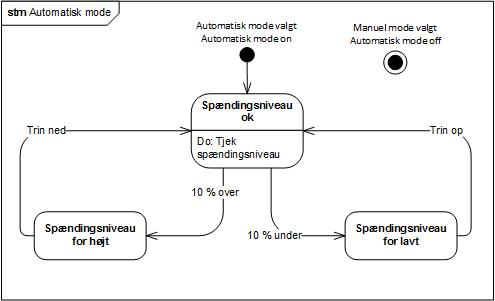
\includegraphics[width=0.8\textwidth]{Figure/STM}
	\caption{Beskrivelse af automatisk mode}
	\label{fig:automode}
\end{figure}

\subsection{Usecase Diagram}

\begin{figure}[H] % (alternativt [H])
	\centering
	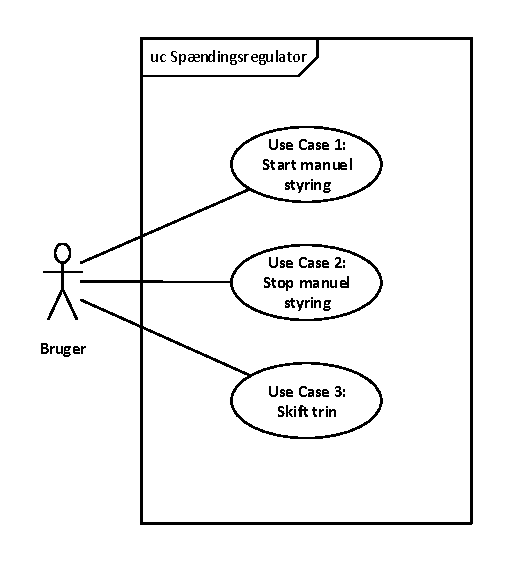
\includegraphics[width=0.5\textwidth]{Figure/UsecaseDiagram}
	\caption{Usecase Diagram}
	\label{fig:UsecaseDiagram}
\end{figure}
Systemet indholder tre usecases, der alle er initieret af brugeren. Den automatiske del af systemet er beskrevet i afsnit \ref{Afsnit: Automatisk mode}.

\subsection{Aktør Beskrivelse}
\textbf{Brugeren} er den primær aktør. En sikkerhedsgodkendt operatør der kan betjene systemet.

\subsection{Usecase 1 - Start manuel styring}
\begin{table}[H]
	\centering
	
	\begin{threeparttable}
		\begin{tabularx}{\linewidth}{ l X }
			\toprule
			\bfseries{Navn:}				& UC1 - Start manuel styring  \\
			\midrule
			\bfseries{Mål:} 				& At sætte systemet i manuel mode \\
			\midrule
			\bfseries{Initiering:} 			& Initieres af brugeren. \\
			\midrule
			\bfseries{Aktører:} 			& Brugeren (Primær) \\
			\midrule
			\bfseries{Samtidige forekomster:} & 1 \\
			\midrule
			\bfseries{Forudsætninger:} 		& At systemet er funktionelt og i automatisk mode\\
			\midrule
			\bfseries{Resultat:} 			& Systemet er i manuel mode \\
			\midrule
			\bfseries{Hovedscenariet:} 	& \\
			
			
			1 	& Brugeren trykker Manuel styring på skærmen.\\
			2	& Systemet skifter til Manuel mode. \\
			3 	& Systemet aktivere manuel skærm. 	\\
			
			\bottomrule
			
		\end{tabularx}
	\end{threeparttable}
	\caption{Fully dressed use case for UC1 - Start manuel styring}
	\label{table:UC1}
\end{table}

\subsection{Usecase 2 - Stop manuel styring}

\begin{table}[H]
	\centering
	
	\begin{threeparttable}
		\begin{tabularx}{\linewidth}{ l X }
			\toprule
			\bfseries{Navn:}				& UC2 - Stop manuel styring  \\
			\midrule
			\bfseries{Mål:} 				& At sætte systemet i automatisk mode \\
			\midrule
			\bfseries{Initiering:} 			& Initieres af brugeren. \\
			\midrule
			\bfseries{Aktører:} 			& Brugeren (Primær) \\
			\midrule
			\bfseries{Samtidige forekomster:} & 1 \\
			\midrule
			\bfseries{Forudsætninger:} 		& At systemet er funktionelt og i manuel mode\\
			\midrule
			\bfseries{Resultat:} 			& Systemet er i automatisk mode \\
			\midrule
			\bfseries{Hovedscenariet:} 	& \\
			
			
			1 	& Brugeren trykker Automatisk styring på skærmen.\\
			2 	& Systemet skifter til Automatisk mode.\\
			3 	& Systemet aktivere automatisk skærm. 	\\		
				
			
			\bottomrule
			
		\end{tabularx}
	\end{threeparttable}
	\caption{Fully dressed use case for UC2 - Stop manuel styring}
	\label{table:UC2}
\end{table}

\subsection{Usecase 3a - Skift trin}

\begin{table}[H]
	\centering
	
	\begin{threeparttable}
		\begin{tabularx}{\linewidth}{ l X }
			\toprule
			\bfseries{Navn:}				& UC3a - Skift trin op  \\
			\midrule
			\bfseries{Mål:} 				& At skifte et trin op på transformeren \\
			\midrule
			\bfseries{Initiering:} 			& Initieres af brugeren. \\
			\midrule
			\bfseries{Aktører:} 			& Brugeren (Primær) \\
			\midrule
			\bfseries{Samtidige forekomster:} & 1 \\
			\midrule
			\bfseries{Forudsætninger:} 		& At systemet er funktionelt og i manuel mode\\
			\midrule
			\bfseries{Resultat:} 			& Transformerens trin er skiftet et trin op \\
			\midrule
			\bfseries{Hovedscenariet:} 	& \\
			
			
			1 	& Brugeren vælger Trin Op på skærmen.\\
			2 	& Systemet skifter et trin op på transformeren.\\
			3 	& Aktuelt trin vises på skærmen.\\
			4 	& Måleværdier opdateres på skærmen.\\		
			
			\bottomrule
			
		\end{tabularx}
	\end{threeparttable}
	\caption{Fully dressed use case for UC3 - Skift trin}
	\label{table:UC3}
\end{table}

\subsection{Usecase 3b - Skift trin}

\begin{table}[H]
	\centering
	
	\begin{threeparttable}
		\begin{tabularx}{\linewidth}{ l X }
			\toprule
			\bfseries{Navn:}				& UC3b - Skift trin ned  \\
			\midrule
			\bfseries{Mål:} 				& At skifte et trin ned på transformeren \\
			\midrule
			\bfseries{Initiering:} 			& Initieres af brugeren. \\
			\midrule
			\bfseries{Aktører:} 			& Brugeren (Primær) \\
			\midrule
			\bfseries{Samtidige forekomster:} & 1 \\
			\midrule
			\bfseries{Forudsætninger:} 		& At systemet er funktionelt og i manuel mode\\
			\midrule
			\bfseries{Resultat:} 			& Transformerens trin er skiftet et trin ned \\
			\midrule
			\bfseries{Hovedscenariet:} 	& \\
			
			
			1 	& Brugeren vælger Trin Ned på skærmen.\\
			2 	& Systemet skifter et trin ned på transformeren.\\
			3 	& Aktuelt trin vises på skærmen.\\
			4 	& Måleværdier opdateres på skærmen.\\			
			
			\bottomrule
			
		\end{tabularx}
	\end{threeparttable}
	\caption{Fully dressed use case for UC3 - Skift trin}
	\label{table:UC3}
\end{table}



% !TEX root = ../../prj4projektdokumentation.tex
\section{Ikke funktionelle krav}
% for spændingsregulator
\begin{table}[H]
	\centering
	\begin{tabular}{|p{4cm}|p{3cm}|p{3cm}|p{3cm}|p{1cm}|}
		\hline
		\textbf{Trintransformer} & \textbf{Handling} & \textbf{Forventet resultat} & \textbf{Resultat} &\textbf{OK} \\\hline
		Nominel spænding på primærsiden er 24VAC & Spændingen på primærsiden måles. & Den målte værdi er 24VAC. &  &  \\\hline
		Nominel spænding på sekundær side er 4, 5 eller 6 VAC afhængig af trin & Spændingen på sekundærsiden måles for hhv. trin 4, 5 og 6. & De målte værdier er 4, 5 og 6V &  & \\\hline
		Skal minimum kunne levere 500mA	. & Strømmen på sekundærsiden måles. & Transformerne kan levere over 500mA &   & \\\hline
	\end{tabular}
	
\end{table} 

% for belastning
\begin{table}[H]
	\centering
	\begin{tabular}{|p{4cm}|p{3cm}|p{3cm}|p{3cm}|p{1cm}|}
		\hline
		\textbf{Belastning} & \textbf{Handling} & \textbf{Forventet resultat} & \textbf{Resultat} &\textbf{OK} \\\hline
		Modstandsværdi på 54$\Omega$ giver spændingsfald på 10\%, når spændingen fra regulatoren er 4V. & Den givne modstand indsættes som belastning, og spændingen herover måles. & Spændingen over belastningen måles til 3,6V. &  &  \\\hline	
	\end{tabular}

	
\end{table}

% for måleenhed
%\begin{table}[htbp]
%	\centering
	\begin{longtable}{|p{4cm}|p{3cm}|p{3cm}|p{3cm}|p{1cm}|}
		\hline
		\textbf{Måleenhed} & \textbf{Handling} & \textbf{Forventet resultat} & \textbf{Resultat} &\textbf{OK} \\\hline
		Måle spændingen ved trinskifteren og forbrugerne mellem 0 og 8 Vrms & Måleenheden testes med spændinger fra 0 til 8Vrms, i intervaller af 500mV. & Korrekt spændingsmåling i hele intervallet. & & \\\hline
		Måle spændingen med en præcision på $\pm$ 5\%& Måleenheden påtrykkes en spænding på 3,5Vrms. Der laves herefter ti målinger& Gennemsnits afvigelsen forventes at være under $\pm$5\%.&  & \\\hline
		Måle strømmen ved trinskifteren og forbrugerne mellem 0 og 500mA& Måleenheden testes med strømme fra 0 til 500mA i intervaller af 50mA&Korrekt strømmåling i hele intervallet.& & \\\hline
		Måle strømmen med en præcision på $\pm$ 5\%&Måleenheden påtrykkes en spænding på 300mVrms (Svarende til 300mA), der laves herefter ti målinger&Gennemsnits afvigelsen forventes at være under $\pm$5\%& & \\\hline
		Måle og beregne power factor med en præcision på $\pm$ 5$\%$&Måleenheden måler power factor over en belastning på distributionslinjen, der sammenlignes med beregnet power factor&Afvigelsen forventes at være under $\pm$ 5\% & & \\\hline
		Beregne THD med en præcision på $\pm$ 5$\%$&Måleenheden påtrykkes en firkantsignal med 1V amplituder og 1V offset. Der sammenlignes med beregnet THD for firkantsignal& Afvigelsen forventes at være under $\pm$ 5\%& & \\\hline
			
	\end{longtable}
	
	
%\end{table}
% !TEX root = ../prj4projektdokumentation.tex

\chapter{Accepttestspecifikation}


% !TEX root = ../../prj4projektdokumentation.tex
% SKAL STÅ I TOPPEN AF ALLE FILER FOR AT MASTER-filen KOMPILERES 

\section{Funktionelle krav}
I dette afsnit beskrives de funktionelle krav for systemet. De dele, hvor en bruger interager med systemet er beskrevet med usecase diagrammer. Den automatiske del er beskrevet og vist vha. et STM diagram.

\subsection{Beskrivelse af automatisk mode}
\label{Afsnit: Automatisk mode}

Når spændingsregulatoren er i automatisk mode, kontrolleres spænding ved forbrugerne. Hvis den spænding er for høj eller lav iht. de 4V skiftes der et trin op eller et trin ned.  
\begin{figure}[htbp] % (alternativt [H])
	\centering
	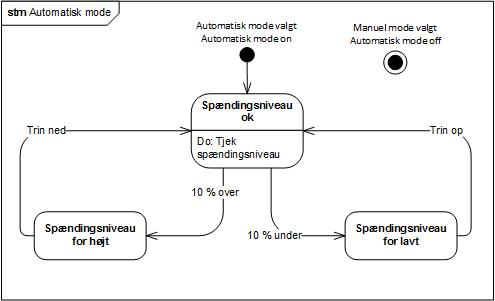
\includegraphics[width=0.8\textwidth]{Figure/STM}
	\caption{Beskrivelse af automatisk mode}
	\label{fig:automode}
\end{figure}

\subsection{Usecase Diagram}

\begin{figure}[H] % (alternativt [H])
	\centering
	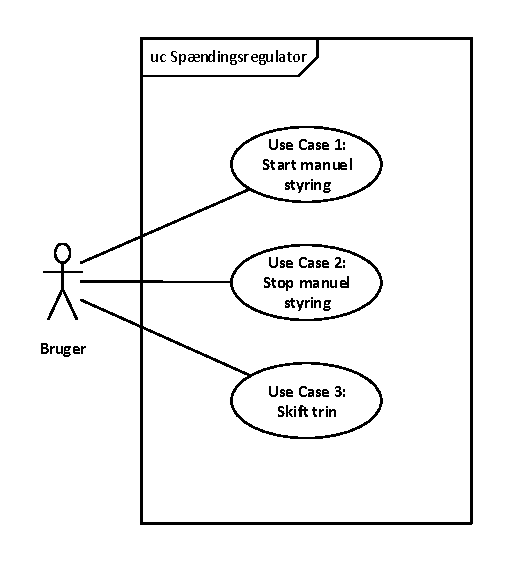
\includegraphics[width=0.5\textwidth]{Figure/UsecaseDiagram}
	\caption{Usecase Diagram}
	\label{fig:UsecaseDiagram}
\end{figure}
Systemet indholder tre usecases, der alle er initieret af brugeren. Den automatiske del af systemet er beskrevet i afsnit \ref{Afsnit: Automatisk mode}.

\subsection{Aktør Beskrivelse}
\textbf{Brugeren} er den primær aktør. En sikkerhedsgodkendt operatør der kan betjene systemet.

\subsection{Usecase 1 - Start manuel styring}
\begin{table}[H]
	\centering
	
	\begin{threeparttable}
		\begin{tabularx}{\linewidth}{ l X }
			\toprule
			\bfseries{Navn:}				& UC1 - Start manuel styring  \\
			\midrule
			\bfseries{Mål:} 				& At sætte systemet i manuel mode \\
			\midrule
			\bfseries{Initiering:} 			& Initieres af brugeren. \\
			\midrule
			\bfseries{Aktører:} 			& Brugeren (Primær) \\
			\midrule
			\bfseries{Samtidige forekomster:} & 1 \\
			\midrule
			\bfseries{Forudsætninger:} 		& At systemet er funktionelt og i automatisk mode\\
			\midrule
			\bfseries{Resultat:} 			& Systemet er i manuel mode \\
			\midrule
			\bfseries{Hovedscenariet:} 	& \\
			
			
			1 	& Brugeren trykker Manuel styring på skærmen.\\
			2	& Systemet skifter til Manuel mode. \\
			3 	& Systemet aktivere manuel skærm. 	\\
			
			\bottomrule
			
		\end{tabularx}
	\end{threeparttable}
	\caption{Fully dressed use case for UC1 - Start manuel styring}
	\label{table:UC1}
\end{table}

\subsection{Usecase 2 - Stop manuel styring}

\begin{table}[H]
	\centering
	
	\begin{threeparttable}
		\begin{tabularx}{\linewidth}{ l X }
			\toprule
			\bfseries{Navn:}				& UC2 - Stop manuel styring  \\
			\midrule
			\bfseries{Mål:} 				& At sætte systemet i automatisk mode \\
			\midrule
			\bfseries{Initiering:} 			& Initieres af brugeren. \\
			\midrule
			\bfseries{Aktører:} 			& Brugeren (Primær) \\
			\midrule
			\bfseries{Samtidige forekomster:} & 1 \\
			\midrule
			\bfseries{Forudsætninger:} 		& At systemet er funktionelt og i manuel mode\\
			\midrule
			\bfseries{Resultat:} 			& Systemet er i automatisk mode \\
			\midrule
			\bfseries{Hovedscenariet:} 	& \\
			
			
			1 	& Brugeren trykker Automatisk styring på skærmen.\\
			2 	& Systemet skifter til Automatisk mode.\\
			3 	& Systemet aktivere automatisk skærm. 	\\		
				
			
			\bottomrule
			
		\end{tabularx}
	\end{threeparttable}
	\caption{Fully dressed use case for UC2 - Stop manuel styring}
	\label{table:UC2}
\end{table}

\subsection{Usecase 3a - Skift trin}

\begin{table}[H]
	\centering
	
	\begin{threeparttable}
		\begin{tabularx}{\linewidth}{ l X }
			\toprule
			\bfseries{Navn:}				& UC3a - Skift trin op  \\
			\midrule
			\bfseries{Mål:} 				& At skifte et trin op på transformeren \\
			\midrule
			\bfseries{Initiering:} 			& Initieres af brugeren. \\
			\midrule
			\bfseries{Aktører:} 			& Brugeren (Primær) \\
			\midrule
			\bfseries{Samtidige forekomster:} & 1 \\
			\midrule
			\bfseries{Forudsætninger:} 		& At systemet er funktionelt og i manuel mode\\
			\midrule
			\bfseries{Resultat:} 			& Transformerens trin er skiftet et trin op \\
			\midrule
			\bfseries{Hovedscenariet:} 	& \\
			
			
			1 	& Brugeren vælger Trin Op på skærmen.\\
			2 	& Systemet skifter et trin op på transformeren.\\
			3 	& Aktuelt trin vises på skærmen.\\
			4 	& Måleværdier opdateres på skærmen.\\		
			
			\bottomrule
			
		\end{tabularx}
	\end{threeparttable}
	\caption{Fully dressed use case for UC3 - Skift trin}
	\label{table:UC3}
\end{table}

\subsection{Usecase 3b - Skift trin}

\begin{table}[H]
	\centering
	
	\begin{threeparttable}
		\begin{tabularx}{\linewidth}{ l X }
			\toprule
			\bfseries{Navn:}				& UC3b - Skift trin ned  \\
			\midrule
			\bfseries{Mål:} 				& At skifte et trin ned på transformeren \\
			\midrule
			\bfseries{Initiering:} 			& Initieres af brugeren. \\
			\midrule
			\bfseries{Aktører:} 			& Brugeren (Primær) \\
			\midrule
			\bfseries{Samtidige forekomster:} & 1 \\
			\midrule
			\bfseries{Forudsætninger:} 		& At systemet er funktionelt og i manuel mode\\
			\midrule
			\bfseries{Resultat:} 			& Transformerens trin er skiftet et trin ned \\
			\midrule
			\bfseries{Hovedscenariet:} 	& \\
			
			
			1 	& Brugeren vælger Trin Ned på skærmen.\\
			2 	& Systemet skifter et trin ned på transformeren.\\
			3 	& Aktuelt trin vises på skærmen.\\
			4 	& Måleværdier opdateres på skærmen.\\			
			
			\bottomrule
			
		\end{tabularx}
	\end{threeparttable}
	\caption{Fully dressed use case for UC3 - Skift trin}
	\label{table:UC3}
\end{table}



% !TEX root = ../../prj4projektdokumentation.tex
\section{Ikke funktionelle krav}
% for spændingsregulator
\begin{table}[H]
	\centering
	\begin{tabular}{|p{4cm}|p{3cm}|p{3cm}|p{3cm}|p{1cm}|}
		\hline
		\textbf{Trintransformer} & \textbf{Handling} & \textbf{Forventet resultat} & \textbf{Resultat} &\textbf{OK} \\\hline
		Nominel spænding på primærsiden er 24VAC & Spændingen på primærsiden måles. & Den målte værdi er 24VAC. &  &  \\\hline
		Nominel spænding på sekundær side er 4, 5 eller 6 VAC afhængig af trin & Spændingen på sekundærsiden måles for hhv. trin 4, 5 og 6. & De målte værdier er 4, 5 og 6V &  & \\\hline
		Skal minimum kunne levere 500mA	. & Strømmen på sekundærsiden måles. & Transformerne kan levere over 500mA &   & \\\hline
	\end{tabular}
	
\end{table} 

% for belastning
\begin{table}[H]
	\centering
	\begin{tabular}{|p{4cm}|p{3cm}|p{3cm}|p{3cm}|p{1cm}|}
		\hline
		\textbf{Belastning} & \textbf{Handling} & \textbf{Forventet resultat} & \textbf{Resultat} &\textbf{OK} \\\hline
		Modstandsværdi på 54$\Omega$ giver spændingsfald på 10\%, når spændingen fra regulatoren er 4V. & Den givne modstand indsættes som belastning, og spændingen herover måles. & Spændingen over belastningen måles til 3,6V. &  &  \\\hline	
	\end{tabular}

	
\end{table}

% for måleenhed
%\begin{table}[htbp]
%	\centering
	\begin{longtable}{|p{4cm}|p{3cm}|p{3cm}|p{3cm}|p{1cm}|}
		\hline
		\textbf{Måleenhed} & \textbf{Handling} & \textbf{Forventet resultat} & \textbf{Resultat} &\textbf{OK} \\\hline
		Måle spændingen ved trinskifteren og forbrugerne mellem 0 og 8 Vrms & Måleenheden testes med spændinger fra 0 til 8Vrms, i intervaller af 500mV. & Korrekt spændingsmåling i hele intervallet. & & \\\hline
		Måle spændingen med en præcision på $\pm$ 5\%& Måleenheden påtrykkes en spænding på 3,5Vrms. Der laves herefter ti målinger& Gennemsnits afvigelsen forventes at være under $\pm$5\%.&  & \\\hline
		Måle strømmen ved trinskifteren og forbrugerne mellem 0 og 500mA& Måleenheden testes med strømme fra 0 til 500mA i intervaller af 50mA&Korrekt strømmåling i hele intervallet.& & \\\hline
		Måle strømmen med en præcision på $\pm$ 5\%&Måleenheden påtrykkes en spænding på 300mVrms (Svarende til 300mA), der laves herefter ti målinger&Gennemsnits afvigelsen forventes at være under $\pm$5\%& & \\\hline
		Måle og beregne power factor med en præcision på $\pm$ 5$\%$&Måleenheden måler power factor over en belastning på distributionslinjen, der sammenlignes med beregnet power factor&Afvigelsen forventes at være under $\pm$ 5\% & & \\\hline
		Beregne THD med en præcision på $\pm$ 5$\%$&Måleenheden påtrykkes en firkantsignal med 1V amplituder og 1V offset. Der sammenlignes med beregnet THD for firkantsignal& Afvigelsen forventes at være under $\pm$ 5\%& & \\\hline
			
	\end{longtable}
	
	
%\end{table}

% !TEX root = ../../prj4projektdokumentation.tex
% SKAL STÅ I TOPPEN AF ALLE FILER FOR AT MASTER-filen KOMPILERES 

\chapter{Arkitektur}

% !TEX root = ../../prj4projektdokumentation.tex
% SKAL STÅ I TOPPEN AF ALLE FILER FOR AT MASTER-filen KOMPILERES 

\section{Blok definitionsdiagram}
Et BDD for spændingsregulator ses på figur \ref{fig:BDDSpaendingsregulator}. På diagrammet ses de overordnet blokke spædingsregulator består af. En beskrivelse af hver blok kan læses under figur \ref{fig:BDDSpaendingsregulator}.

\begin{figure}[htbp] % (alternativt [H])
	\centering
	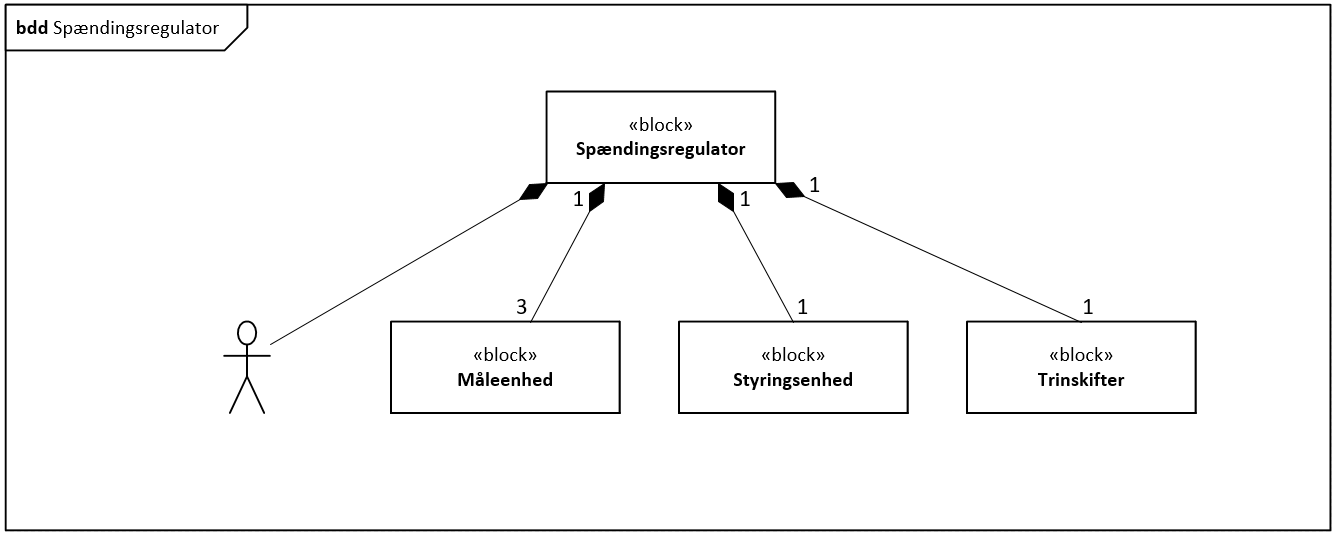
\includegraphics[width=0.9\textwidth]{Figure/BDDSpaendingsregulator}
	\caption{BDD Spændingsregulator}
	\label{fig:BDDSpaendingsregulator}
\end{figure}

\textbf{Måleenhed} står for at måle spænding, strøm og faseforskydningen herimellem. Ligeledes skal denne kunne måle indeholdet af harmoniske frekvenser. Den består af hardware til måling af de nævnte parametre og en PSoC 5. På enheden ligger også en del af behandlingen af rådataet, så dette kan formidles til styringsenheden.

\textbf{Styringsenhed} har til opgave at styre trinskifteren ud fra de data den får fra målenehderne. Den består af en PLC, tl styringen og et HMI, der skal give en bruger overblik over status for distributionslinjen.

\textbf{Trinskifter} er en enhed der kan skifte trin på transformeren ud fra et signal fra styringsenheden. Den består altå af en kontakt for hvert trin, der kan kontrolleres af styringsenheden.
% !TEX root = ../../prj4projektdokumentation.tex
% SKAL STÅ I TOPPEN AF ALLE FILER FOR AT MASTER-filen KOMPILERES 

\section{Intern blok diagram}
På figur \ref{fig:IBDSp} og figur \ref{fig:IBDSt} ses IBD for henholdsvis Spændingsregulator og Styringsenhed. På diagrammerne ses de interne forbindelser i systemet. Under figurne er tilhørende signalbeskrivelser, se tabel \ref{tab:SignalbeskrivelseSp} og tabel \ref{tab:SignalbeskrivelseSt}, der uddyber diagrammerne nærmere.

\begin{figure}[htbp] % (alternativt [H])
	\centering
	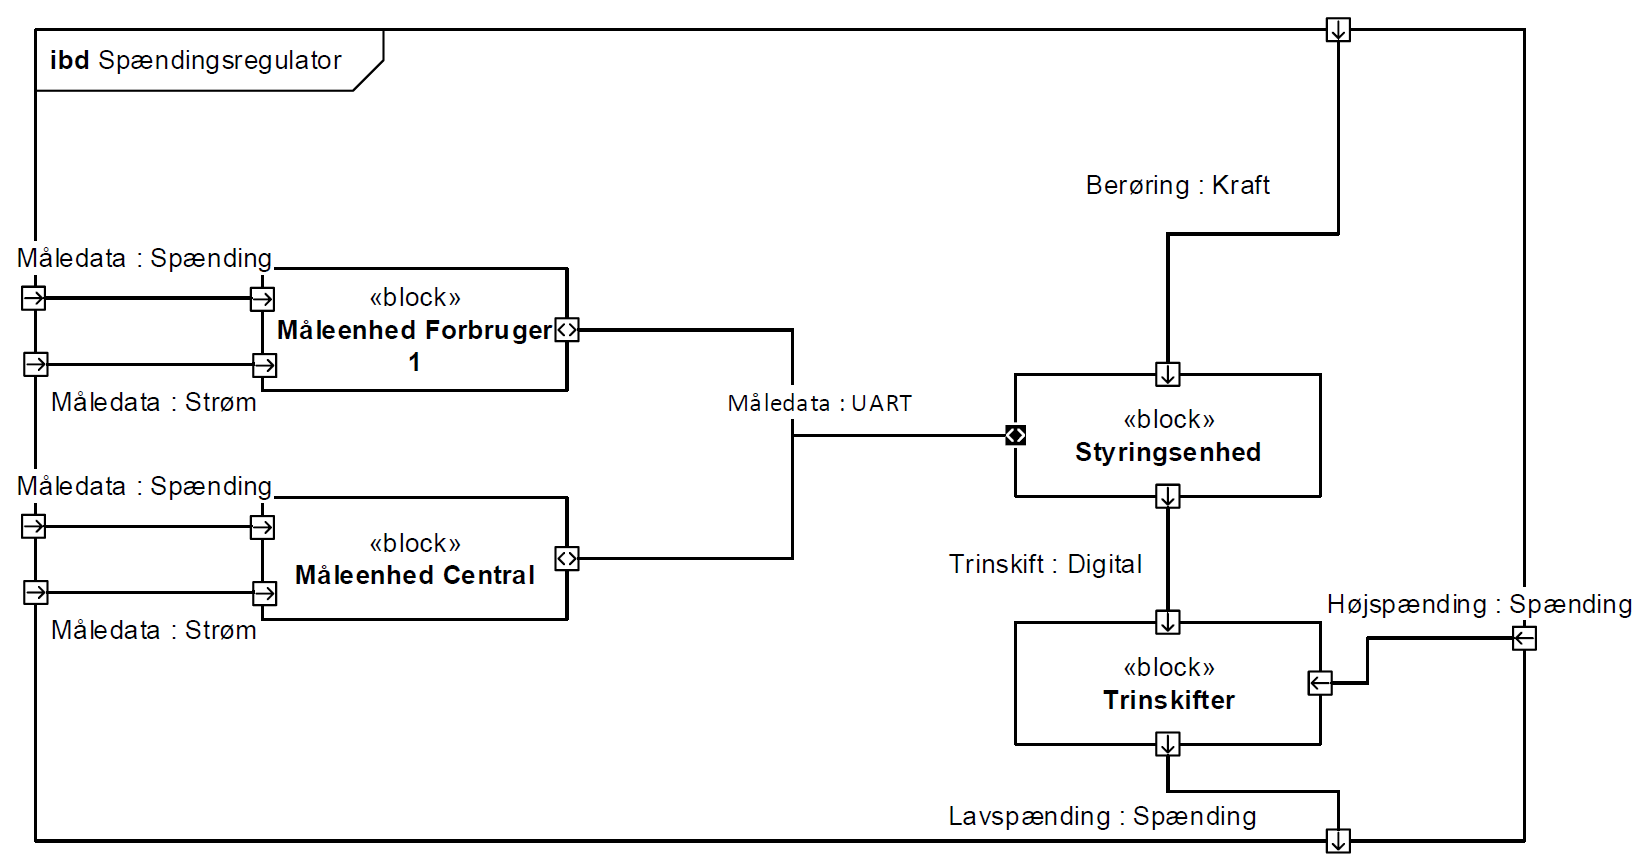
\includegraphics[width=0.8\textwidth]{Figure/IBDSpaendingsregulator1}
	\caption{IBD for Spændingsregulator}
	\label{fig:IBDSp}
\end{figure}

\begin{table}[H]
	\centering
	\begin{tabular}{|l|l|l|l|p{4cm}|}
		\hline
		\textbf{Blok} & \textbf{Navn} & \textbf{Type} & \textbf{Signal} & 
		\textbf{Beskrivelse} \\\hline
		
		\multirow{3}{*}{Måleenhed} 
		& Måledata & Spænding & In & Måledata er spændingsniveauet på distributionslinjen. \\\hhline{~----} 
		& Måledata & Strøm & In & Måledata er strømniveauet på distributionslinjen. \\\hhline{~----} 
		& Måledata & UART & InOut & UART forbindelse til Styringsenhed \\\hline
		
		\multirow{3}{*}{Styringsenhed} 
		& Måledata & UART & Inout & UART forbindelse til Måleenhed \\\hhline{~----} 
		& Berøring & Kraft & In & Tryk på Brugergrænseflade \\\hhline{~----} 
		& Trinskift & Digital & Out & Trinskift er en digital kommando til Trinskifter \\\hline
		
		\multirow{3}{*}{Trinskifter} 
		& Trinskift & Digital & In & Trinskift er en digital kommando fra Styringsenhed. \\\hhline{~----} 
		& Højspænding & Spænding & In & Er spændingen på højspændingssiden af tranformeren. \\\hhline{~----} 
		& Lavspænding & Spænding & Out & Er spændingen på lavspændingssiden af transformeren. \\\hline
	\end{tabular}
	\caption{Signalbeskrivelse for Spændingsregulator}
	\label{tab:SignalbeskrivelseSp}
	
\end{table}


\begin{figure}[htbp] % (alternativt [H])
	\centering
	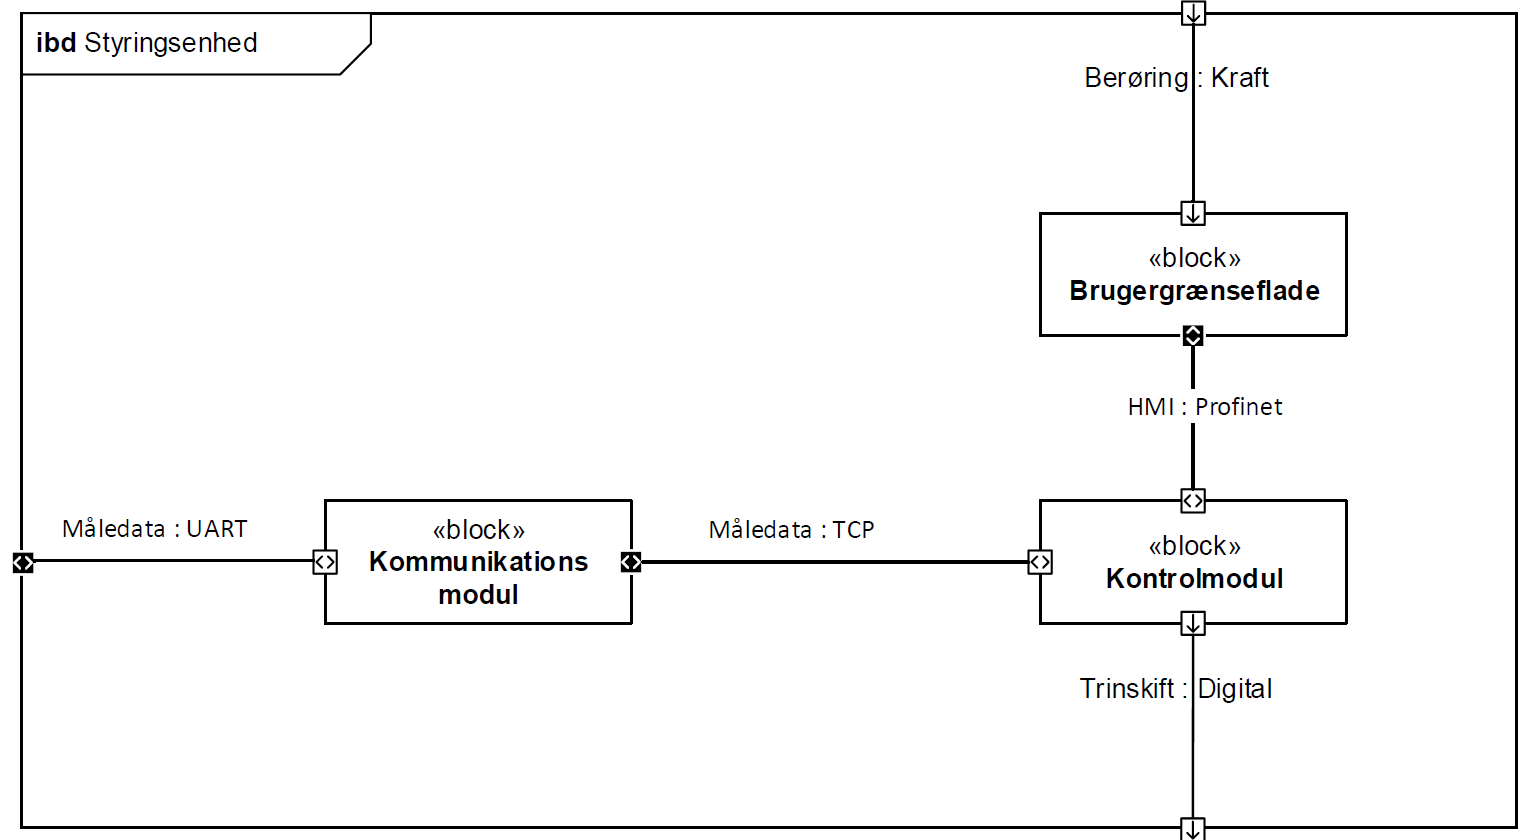
\includegraphics[width=0.8\textwidth]{Figure/IBDStyringsenhed1}
	\caption{IBD for Styringsenhed}
	\label{fig:IBDSt}
\end{figure}

\begin{table}[H]
	\centering
	\begin{tabular}{|l|l|l|l|p{4cm}|}
		\hline
		\textbf{Blok} & \textbf{Navn} & \textbf{Type} & \textbf{Signal} & 
		\textbf{Beskrivelse} \\\hline
		
		\multirow{2}{*}{Brugergrænseflade} 
		& Berøring & Kraft & In & Tryk på Brugergrænseflade \\\hhline{~----} 
		& HMI & Profinet & InOut & Forbindelse til Kontrolmodul \\\hline
		
		\multirow{3}{*}{Kontrolmodul} 
		& HMI & Profinet & InOut & Forbindelse til Brugergrænseflade \\\hhline{~----} 
		& Trinskift & Digital & Out & Trinskift er en digital kommando til Trinskifter \\\hhline{~----} 
		& Måledata & TCP & InOut & TCP forbindelse til Kommunikationsmodul \\\hline
		
		\multirow{2}{*}{Kommunikationsmodul} 
		& Måledata & TCP & InOut & TCP forbindelse til Kontrolmodul \\\hhline{~----} 
		& Måledata & UART & InOut & UART forbindelse til Måleenhed \\\hline
	\end{tabular}
	\caption{Signalbeskrivelse for Styringsenhed}
	\label{tab:SignalbeskrivelseSt}
	
\end{table}


\newpage
% !TEX root = ../../prj4projektdokumentation.tex
% SKAL STÅ I TOPPEN AF ALLE FILER FOR AT MASTER-filen KOMPILERES 

\section{Allokeringsdiagram}
På figur \ref{fig:Allokering} ses allokeringsdiagram for spændningsregulatoren. Diagrammet er lavet for at danne overblik over softwaren, derfor er analog moduler undladt. Styringsenheden laver et output til trin transformeren og Måleenehederne får input fra belastninger. Det er heller ikke vist på diagrammet. Diagrammet viser hvilke platforme de logiske blokke skal laves på, og hvordan kommunikationen er mellem blokkene

\begin{enumerate}
	\item Styringsenheden allokeres på en PLC
	\item Brugergrænsefladen allokeres på en HMI skærm
	\item Måleenhederne allokeres på PSoCs
\end{enumerate}   

\begin{figure}[htbp] % (alternativt [H])
	\centering
	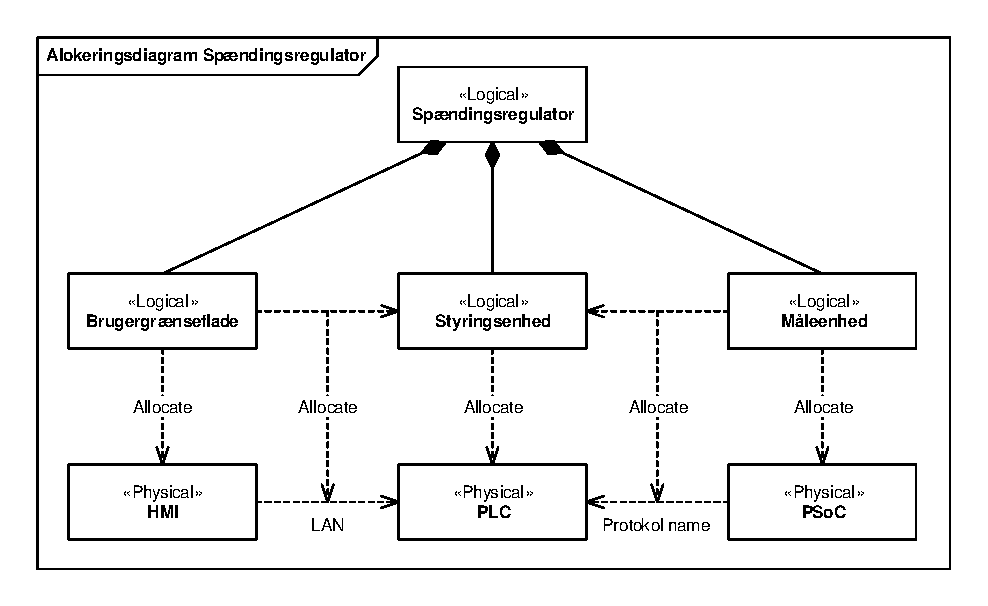
\includegraphics[width=0.9\textwidth]{Figure/Allokering}
	\caption{Allokeringsdiagram for spændingsregulator}
	\label{fig:Allokering}
\end{figure}
% !TEX root = ../../prj4projektdokumentation.tex
% SKAL STÅ I TOPPEN AF ALLE FILER FOR AT MASTER-filen KOMPILERES 

\section{Brugergrænseflade}
(Beskrivelse af skærm på PLC’en) \\
\subsection{Automatisk mode}
\begin{figure}[H] % (alternativt [H])
	\centering
	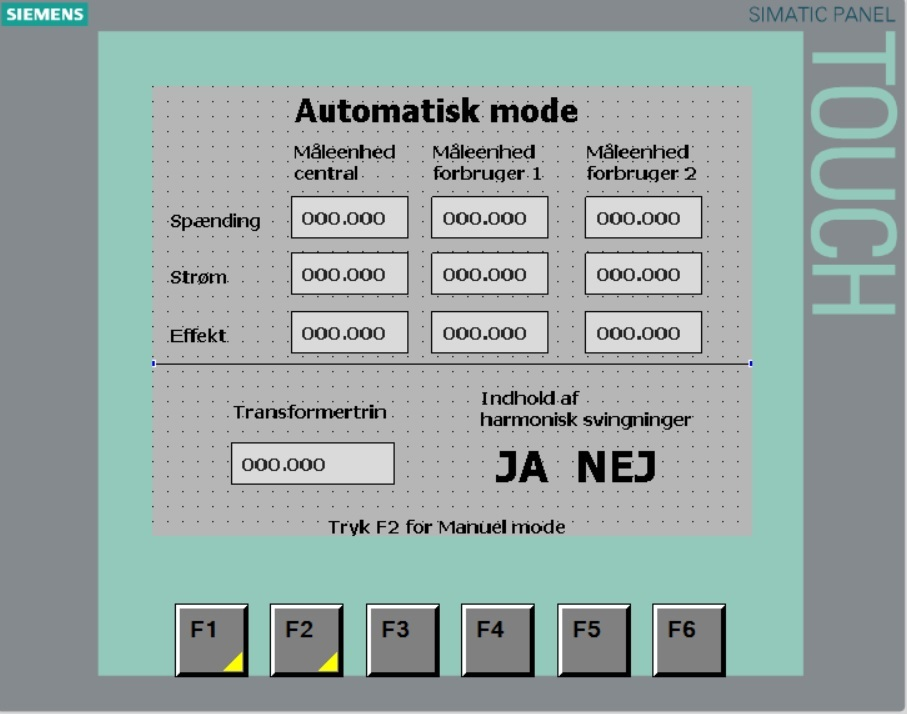
\includegraphics[width=0.9\textwidth]{Figure/HMIAutomatiskMode}
	\caption{HMI Automatisk mode}
	\label{fig:HMIAutomatikMode}
\end{figure}



\subsection{Manuel mode}
\begin{figure}[H] % (alternativt [H])
	\centering
	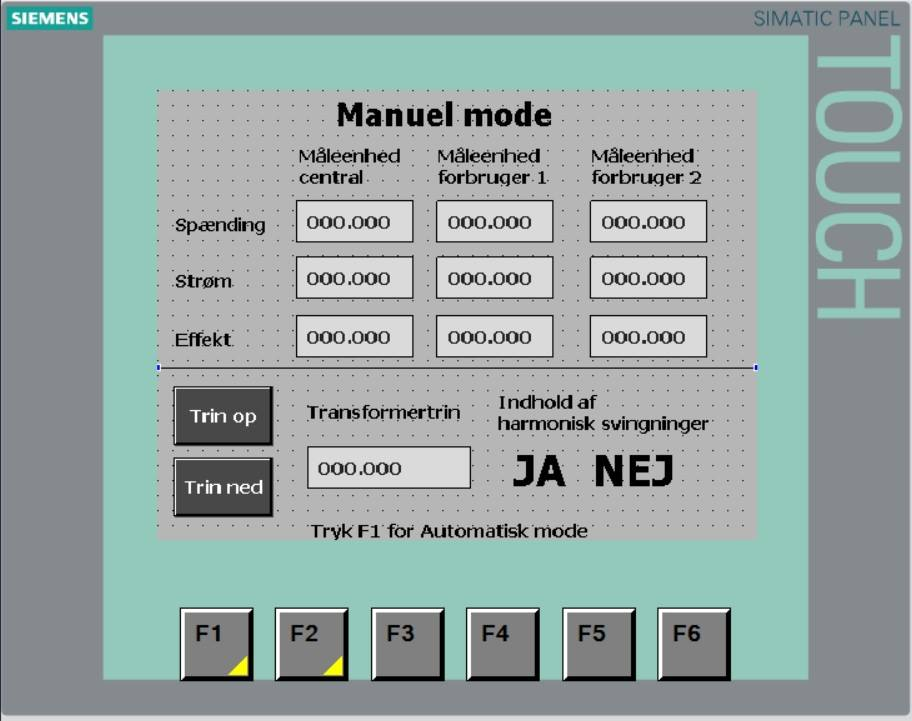
\includegraphics[width=0.9\textwidth]{Figure/HMIManuelMode}
	\caption{HMI Manuel mode}
	\label{fig:HMIManuelMode}
\end{figure}
% !TEX root = ../prj4projektdokumentation.tex
% SKAL STÅ I TOPPEN AF ALLE FILER FOR AT MASTER-filen KOMPILERES 

\chapter{Foranalyse}

\section{Valg af transformer}
Emir udleverede to transformere. Den ene er der ingen mærkeplade og ledningerne var alle samme farve. Den anden har mærkeplade og forskellige farvet ledninger. De to transformere blev begge undersøgt i laboratoriet, med en 18VAC på primærside, derefter måltes spændingen på de forskellige trin. Transformeren uden mærkeplade hoppede små skridt fra ca 3 - 4.5V, hvor transformeren med mærkeplade havde skridt på 1 V fra 0 til 8V. Gruppen blev enige om at det var ligegyldigt om det var små eller store skridt transformeren hoppede, bare protypen blev lavet så den passede til transformeren. Det blev derfor besluttet at anvende transformeren med mærkeplade og forskellige farvet ledninger. 

\section{Valg af styringsenhed}
Det er besluttet at lave Styringsenheden på en PLC, dette gøres for at realisere, hvordan det ville laves i virkeligheden. Alternativt kunne det laves på en PSOC eller Arduino, men da der på dette semester er undervisning i PLC styring virker det derfor oplagt.

\section{Overvejelser omkring måleenhederne}
Det var først tænkt at der kunne laves eller købes nogle sensorer som skulle tilsluttes PLC'en. PLC'en kan dog ikke måle hurtigt nok på AC forbindelser til at få et reelt billed af signalet. Derfor bruges PSOC til at måle og sample signalet og sende det derfra til PLC'en.

\section{Protokoller}




% !TEX root = ../../prj4projektdokumentation.tex

\chapter{Kommunikationsprotokoller}
\label{ch:KomProtokol}

\section{TCP protokol}
\label{sec:TCPprotokol}
Mellem kommunikationsmodulet og kontrolmodulet er anvendt en TCP protokol. TCP er valgt, da systemet ikke kræver hurtig, men derimod en meget pålidelig datatransmission. PLC'en anvender stikstandarden RJ-45 og har mulighed for at kommunikere med hastighederne 10/100 Mb/s. Komponenterne i systemet tillader 100 Mb/s.
PLC'en er opsat som client, der forespørger data fra Arduinoen, som svarer med det forespurgte data. Kommunikation over TCP forbindelsen anvender protokollen vist på figur \ref{fig:TCPprotokol}.

\begin{figure}[H] % (alternativt [H])
	\centering
	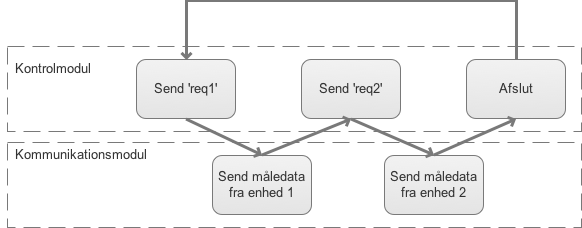
\includegraphics[width=0.7\textwidth]{Figure/TCPprotokol}
	\caption{Protokol for kommunikation mellem kommunikationsmodul og kontrolmodul}
	\label{fig:TCPprotokol}
\end{figure}

Måledata består af otte bytes i sæt af to bytes. De fire sæt dækker over måleværdier for henholdsvis, strøm, spænding, powerfactor og THD. Yderligere information om TCP kommunikationen kan findes i afsnit \ref{sec:TCPkommunikation} TCP kommunikation og \ref{sec:Kommunikationsmodul} Kommunikationsmodul.

\section{UART protokol}
\label{sec:UARTprotokol}
UART protokollen anvendes mellem Måleenheden og Styringsenheden. Opsætning af UART forbindelse overholder indstillingerne i Tabel \ref{tab:UARTprotokol}. Data som transmitteres over UART forbindelsen sendes i pakker af 8-bit. Da værdier for strøm, spænding, power factor og THD er uint16 værdier, skal der for hver værdi sendes to pakker, henholdsvis MSB og LSB. 

Kommunikation over UART forbindelsen skal overholde følgende protokol, se Figur \ref{fig:UARTprotokol}.
\begin{figure}[H] % (alternativt [H])
	\centering
	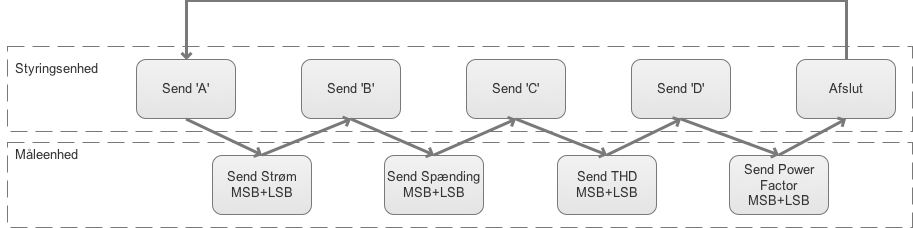
\includegraphics[width=\textwidth]{Figure/UARTprotokol}
	\caption{Protokol for kommunikation mellem Måleenhed og Styringsenhed}
	\label{fig:UARTprotokol}
\end{figure}

\begin{table}[h]
	\centering
	\caption{UART protokol}
	\label{tab:UARTprotokol}
	\begin{tabular}{@{}lll@{}}
		\toprule
							& Indstilling       		& Bemærkning \\ \midrule
		Mode       		& Full UART (Rx+Tx) &            \\
		BaudRate 	  & 9600             		 &            \\
		DataBits    	& 8             			    &            \\
		ParityType 	  	& None     			         &            \\
		Stopbits    	& 1               				  &            \\
		Flowcontrol 	& None         		     &           \\ \hline
	\end{tabular}
\end{table}

% !TEX root = ../../prj4projektdokumentation.tex

\chapter{Design}

\section{Distributionslinje}
På baggrund af foranalysen er længden af distributionslinjen, der ønskes simuleret, valgt til 60 km. Ud fra datablade for den valgte kabeltype ses at der er vil være 0,1 $\omega$ /km og 0,219 mH/km. For at kunne simulere disse værdier er opbygget et kredsløb med 6,2 $\omega$ modstand i serie med en 13,6 mH spole. 




% !TEX root = ../../prj4projektdokumentation.tex

\section{Belastning}

Med denne distributionslinje og med trinskifteren, der står på 4V trinnet, kan det beregnes hvilken belastning, der vil medføre, at spændingen hos forbrugeren falder til under 10 \% \\ af 4V. Kredsløbet og beregningen ses nedenfor.

\begin{figure}[htbp] % (alternativt [H])
	\centering
	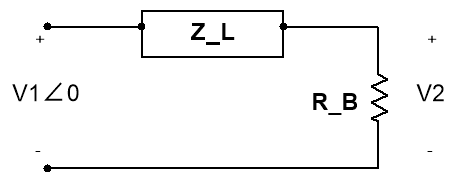
\includegraphics[width=0.4\textwidth]{Figure/Belastningberegning}
	\caption{Kredsløb til beregning af belastning}
	\label{fig:Belastningberegning}
\end{figure}

Først bruges spændingsdelerformlen

\begin{align}
	V2=V1\cdot\frac{R_B}{Z_L+R_B}
\end{align}

\begin{align}
	0,9\cdot\vert V1 \vert = \vert V1\cdot\frac{R_B}{Z_L+R_B} \vert = V1\cdot\frac{R_B}{R_L+jX_L+R_B}
\end{align}

\begin{align}
0,9= \vert \frac{R_B}{R_L+jX_L+R_B} \vert
\end{align}

\begin{align}
	0,9\cdot\vert R_L+jX_L+R_B \vert = \vert R_B \vert
\end{align}

\begin{align}
0,9\cdot\sqrt{(R_L+R_B)^2+X_L^2}=R_B
\end{align}

\begin{align}
(R_L+R_B)^2+X_L^2=\frac{R_B^2}{0,81}
\end{align}

\begin{align}
R_L^2+R_B^2+2\cdot R_L\cdot R_B+X_L^2=\frac{R_B^2}{0,81}
\end{align}

\begin{align}
R_B^2\cdot (1-\frac{1}{0,81})+2\cdot R_L\cdot R_B+X_L^2=0
\end{align}

Værdier indsættes og herved fås:

\begin{align}
R_B^2\cdot (-0,24) +12,4\cdot R_B+18,23=0
\end{align}

Andengrads ligning løses og derved findes den modstandsværdi, der vil give et spændingsfald på 10\%.

\begin{align}
R_B=\frac{-12,4\pm\sqrt{153,76-4\cdot(-0,24)\cdot18,23}}{-0,24\cdot 2}=\frac{-12,4\pm 13,1}{-0,47}=54,3 \Omega
\end{align}

Denne modstandsværdi i det viste kredsløb og med den valgte distributionslinje vil resultere i at spændingen falder under det ønskede niveau som er 4V. Der tages derfor udgangspunkt i denne værdi, men efterfølgende vil belastninger bestemmes ud fra simuleringer i værktøjet Multisim. 

Til implementering af belastninger/forbrugere er på baggrund af foregående beregninger valgt modstande i intervallet 16 $\Omega$ til 100 $\Omega$. Belastninger er placeret i parallel og til hver belastning hører en kontakt, således der let kan skiftes mellem forskellige værdier. Der er desuden monteret pin til forbindelse til distributionslinje og bananstik til forbindelse til 0V på transformeren. Yderligere er der for hver belastning monteret en 1 $\Omega$ modstand således Måleenheden kan overvåge tilstanden hos hver forbruger. Det færdige print med belastninger ses på figur \ref{fig:Belastning1}

\begin{figure}[H] 
	\centering
	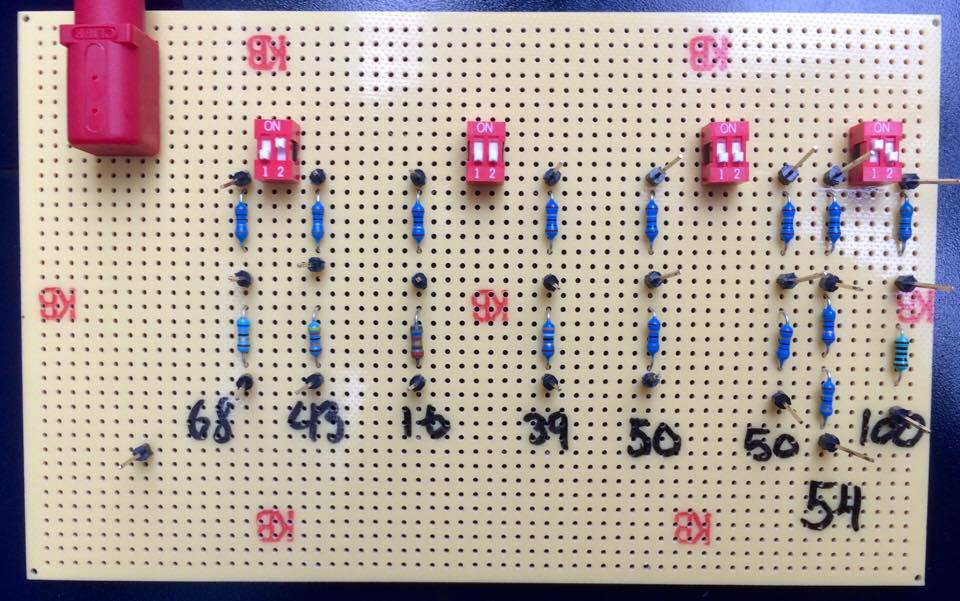
\includegraphics[width=0.7\textwidth]{Figure/Belastningskreds}
	\caption{Færdigt print med belastninger/forbrugere}
	\label{fig:Belastning1}
\end{figure}




% !TEX root =../prj4projektrapport.tex

\section{Trinskifter}

Ved projektets start fik gruppen udleveret en trintransformer\footnote{Projektdokumentation, 6.1, Valg af transformer}. Denne transformer har på primærside 24V og trin af 1V fra 0-8V på sekundærside. Disse forhold afgjorde skaleringen af systemet, se bilag C3 og C4 for billeder af transformer og tilhørende mærkeplade. 

De forskellige trin og dermed spændingsniveauer på sekundærside af transformeren er bestemt af antallet af tilkoblede viklinger. Det ønskede spændingsniveau hos forbrugeren er valgt til 4V, og det er i systemet muligt at skifte mellem trin 4V,5V og 6V på trintransformeren. Disse tre trin gør at muligt at holde spændingen hos forbrugeren på $\pm$10$\%$ af 4V, når belastningen varierer.

\subsection{Design og implementering af relækredsløb}
Til at styre tilkoblingen af trin på transformeren er der designet et relækredsløb. Relæerne er sat til Normally Open og virker som kontakter, der slutter, når relæet trækker. Relæerne skal styres af en PLC, og skal derfor kunne holde til et 24VDC styresignal \footnote{Projektdokumentation, 8.4, Trinskifter}. Det færdige print med relæer ses på figur \ref{fig:Relae}. De sorte banastik kobles til henholdsvis trin 4V,5V og 6V på transformeren. Øverst til ses pin, der kobles til Distributionslinjen. De tre pins nederst til venstre er til styresignal fra PLC og den fjerde er stelforbindelse for PLC. 

\begin{figure}[H]
	\centering
	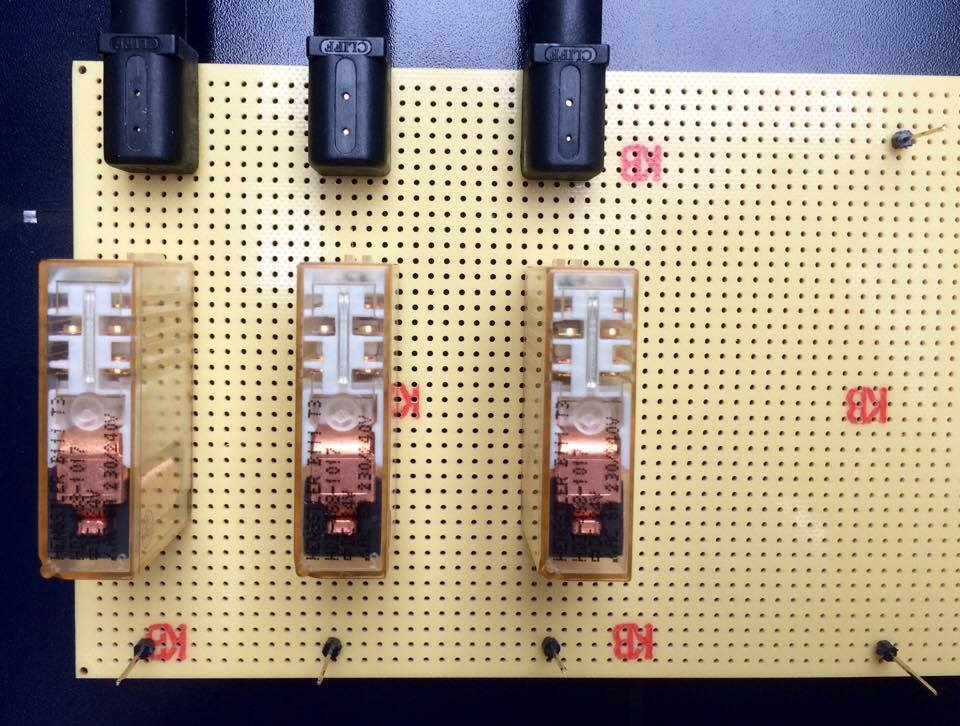
\includegraphics[width=0.6\textwidth]{figure/Relaekredsl}
	\caption{Færdigt print med relæer}
	\label{fig:Relae}
\end{figure}

\subsection{Implementering af Trinsskifter}

Trinskifter består af trintransformer og relækredsløb. På figur \ref{fig:Trinskift} ses implementeringen af denne samt kobling til PLC, Distributionslinje og belastninger.

\begin{figure}[H]
	\centering
	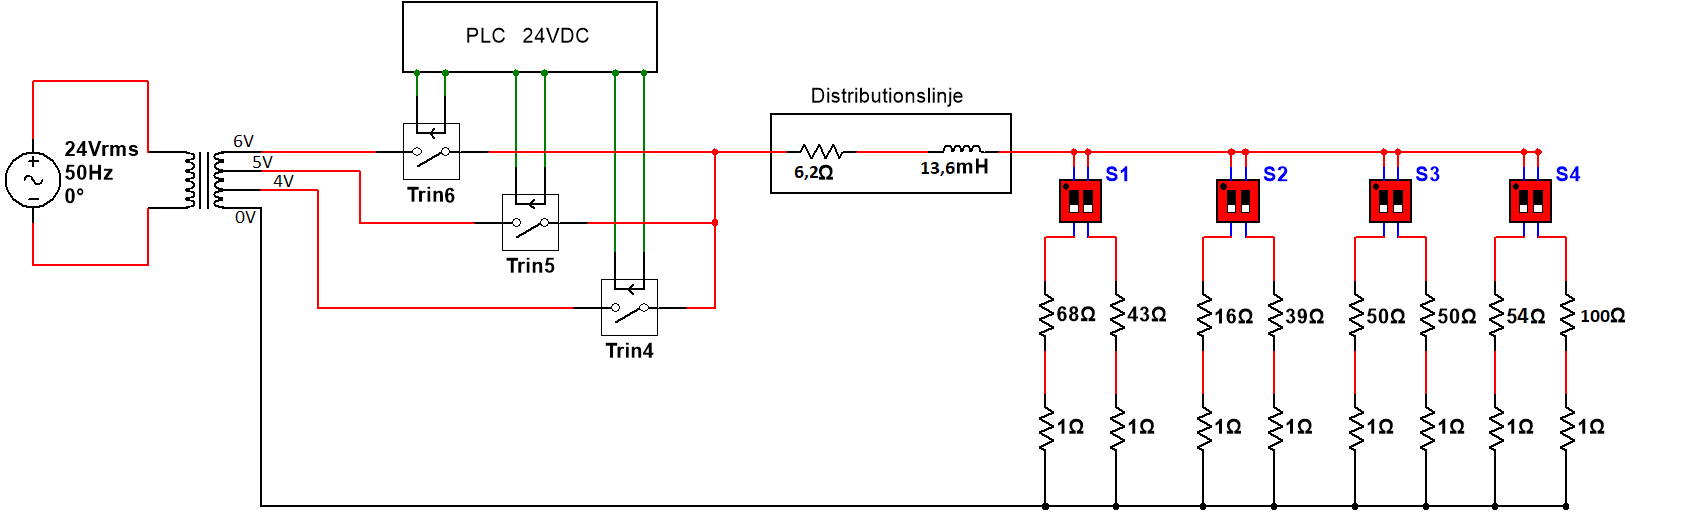
\includegraphics[width=0.8\textwidth]{figure/Trinskiftertegning2}
	\caption{Kredsløbstegning af Distributionslinje, belastninger og Trinskifter}
	\label{fig:Trinskift}
\end{figure}


% !TEX root =../prj4projektrapport.tex

\section{Modultest}


\chapter{Design af Måleenhed}
% !TEX root = ../../prj4projektdokumentation.tex

\section{Indledning}
I dette afsnit beskrives, hvordan Måleenheden er opbygget. Måleenheden er designet til at kunne måle centralt og decentralt, på projektets simulering af transmissionslinje og forbrugere. Der er på netværket forberedt til at der kan tilsluttes måleenheder på forbrugerne. Spændingen kan måles direkte over forbrugeren. På hver forbruger er der tilsluttet 1 1$\Omega$ modstand i serie. På denne modstand måles spændingen, som vil være proportional med strømmen i systemet. Måleenheden er hovedsageligt software, der sampler og udregninger rms, power factor og THD. Der er dog også lavet hardware til at bearbejde signalerne inden PSOC'en.


\section{Hardware}
\subsection{Indledning}
Måleenhedens hardware skal kunne dæmpe spændingen og forstærke strømmen så det ligger inden for PSOC'ens ADC spændingsområde. ADC kan sample signaler mellem 0 og 5Vpp, Det betyder at signalernes offset skal ændres til 2,5V.

\subsection{Diagram}
På figur \ref{fig:MaalDiagram} ses diagrammet for det hardware der bruges til at dæmpe spændingen, forstærke strømmen og hæve offsettet.

\begin{figure}[H] % (alternativt [H])
	\centering
	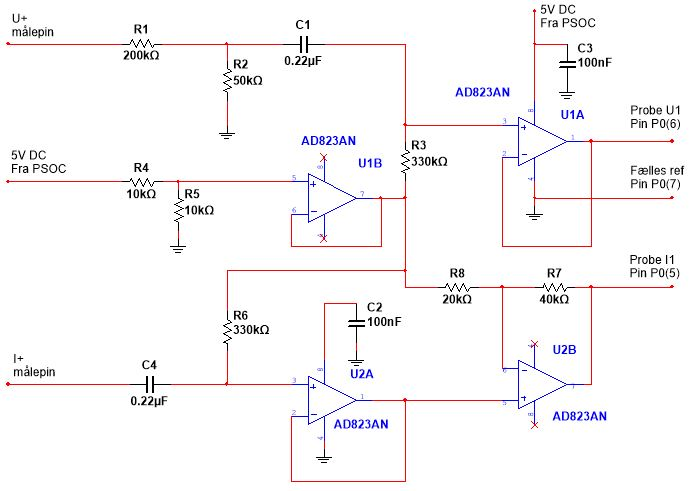
\includegraphics[width=\textwidth]{Figure/MaalHardware}
	\caption{Hardware diagram}
	\label{fig:MaalDiagram}
\end{figure}


\subsubsection{Spændingsmåler}
For at kunne måle den maksimale spænding på 8V rms, dvs.

\begin{align}
Vpp = 8V*\sqrt{2} = 11,3Vpp
\end{align}

Den mindste dæmpning skal derfor være:

\begin{align}
min\_daemp = \dfrac{11.3}{5} = 2,26 gange
\end{align}

Dette er valgt realiseret med en spændingsdeler ved R1 og R2. De dæmper med 3 gange og niveauet kommer derfor indenfor marginen.
Derefter bliver offsettet hævet ved hjælp af signalet fra U1B. Til sidst føres signalet gennem spændingsfølgeren U1A for at sikre spændingen.

\subsubsection{Strømmåling}
Strømmålingen laves ved at måle spændingen over en 1$\Omega$ modstand. Modstanden sidder placeret ved belastningen. Iht. ohmslov vil det give strømmen i systemet
.
\begin{align}
	I = \dfrac{U}{1\Omega} = U
\end{align}

Første Opamp U2A ved strømmålingen bruges til at hæve DC offset til 2,5V. Opamp U2B bruges til at forstærke strømmen så der kommer bedre præcision på målingen. Den maskimale forstærkning, for at den passe indenfor PSOC'ens ADC sample område bliver derfor:

Den maksimale Ipp der vil kunne måles:
\begin{align}
Ipp = 0,5*\sqrt{2} = 0,71A
\end{align}

Maksimale forstærkning:
\begin{align}
maks\_forstaerkning = \dfrac{5}{0,71} = 7
\end{align}
Denne forstærkning ses realiseret vha. modstand R7 og R8.  

\subsubsection{PSOC tilslutning}
Spændingen og strømmen bliver målt til den fælles nul i systemet, der bliver koblet på hardwarens stel forbindelse. Spænding, strøm og stel forbindelsen tilsluttes PSOC'en, som vist på figur \ref{fig:MaalDiagram}.





% !TEX root = ../../prj4projektdokumentation.tex

\section{Software}

I dette afsnit vil softwaren for Måleenheden blive beskrevet. Herunder beskrivelser af det overordnede flow i koden, samt en uddybning af udviklede funktioner til sampling, Fourier-udregninger og Total Harmonic Distortion. 

\subsection{Overordnet beskrivelse}

Softwaren til Måleenheden er allokeret på PSOC. Det overordnede flow i koden er beskrevet i Figur \ref{fig:MEflowchart}. 

Som det første åbnes der for globale interrupts, så der kan modtages receive-interrupts fra UART forbindelsen til Styringsenheden. Herefter inittieres de anvendte blokke i PSOC, herunder ADC og UART. 

Efter initialiseringen går koden i et uendeligt loop hvor der ikke er nogen aktivitet.  Her ventes der på et receive-interrupt fra UART forbindelsen. Ifølge protokollen for kommunikation mellem Måleenhed og Styringsenhed, se kapitel \ref{ch:KomProtokol}, forventes det at rækkefølgen af karakterer der modtages er "A-B-C-D". Denne rækkefølge er afgørende, da sampling og udregning, først starter ved modtagelse af karakteren 'A'. 

Når udregningerne er udført, sendes den udregnede RMS-værdi for den målte strøm, over UART-forbindelsen. Værdien, som er en 16bit integer, sendes i to bytes, henholdsvis MSB og LSB. 

Når de to bytes er sendt til Styringsenheden forlades interruptrutinen, og koden returnerer til det uendelig loop, hvor der ventes på at modtage den næste karakter i rækkefølgen. 

Ved modtagelse af de efterfølgende karakterer sendes værdierne for henholdsvis spænding, THD og Power Factor. 


\begin{figure}[H] % (alternativt [H])
	\centering
	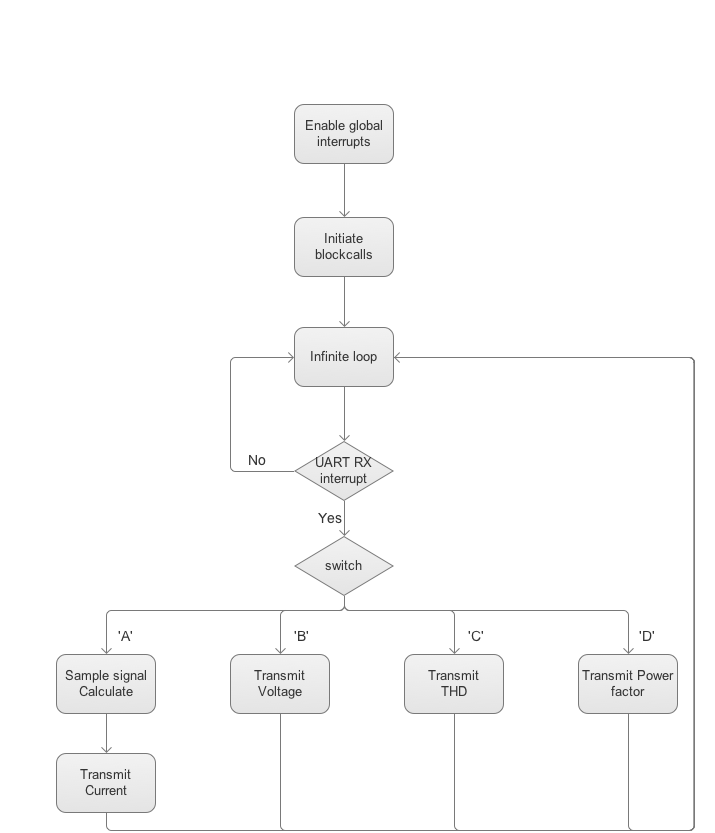
\includegraphics[width=0.7\textwidth]{Figure/MEflowchart.png}
	\caption{Overordnet flowchart for software på Måleenhed}
	\label{fig:MEflowchart}
\end{figure}


% !TEX root = ../../prj4projektdokumentation.tex
% !TEX root = ../../prj4projektdokumentation.tex
% !TEX root = ../../prj4projektdokumentation.tex
% !TEX root = ../../prj4projektdokumentation.tex
% !TEX root = ../../prj4projektdokumentation.tex

\subsection{Kalibrering af måleenhed.}

Efter test af funktionaliteten af Måleenheden laves en kalibrering, for at fjerne det offset, som er opstået i forbindelse med forstærkning/dæmpning af signal i hardwaren. 

\subsubsection{Måleopstilling}

Til kalibrering af måleenheden er anvendes en funktionsgenerator, til at lave sinussignalet, som forbindes direkte til måleenheden. Til korrekt måling af spændingsværdier anvendes oscilloskop, som her antages for værende ideel. Måleenheden er tilsluttet en PC og kører i debug-mode, så værdierne for strøm og spænding kan aflæses. 
\begin{figure}[H]
	\centering
	\begin{minipage}[b]{0.48\textwidth}
		\centering
		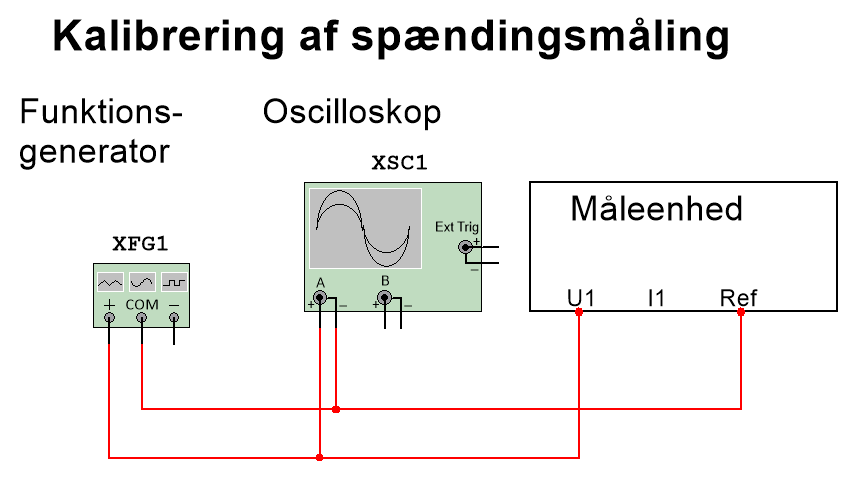
\includegraphics[width=1.00\textwidth]{Figure/MEkalibreringU} % Venstre billede
	\end{minipage}
	\hfill
	\begin{minipage}[b]{0.48\textwidth}
		\centering
		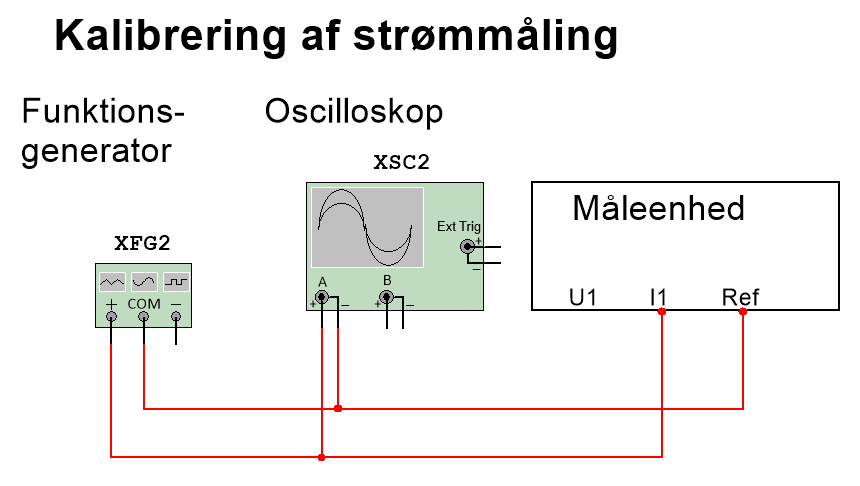
\includegraphics[width=1.00\textwidth]{Figure/MEkalibreringI} % Højre billede
	\end{minipage}
	\\ % Figurtekster og labels
	\begin{minipage}[t]{0.48\textwidth}
		\caption{Måleopstilling for kalibrering af spændingsmåling} % Venstre figurtekst og label
		\label{fig:MEkalibreringU}
	\end{minipage}
	\hfill
	\begin{minipage}[t]{0.48\textwidth}
		\caption{Måleopstilling for kalibrering af strømmåling} % Højre figurtekst og label
		\label{fig:MEkalibreringI}
	\end{minipage}
\end{figure}

\subsubsection{Fremgangsmåde}

Der laves to måleserier, for henholdsvis spænding- og strømmåling. Strømmålingen er baseret på en spændingsmåling over en $1\Omega$ modstand, hvilket betyder at spændingsfaldet over modstanden lig med strømmen. Derfor kalibreres strømmålingen med et spændingssignal, på samme måde som spændingsmålingen. Måleenheden er lavet til at måle en spænding mellem 0-8Vrms og en strøm mellem $\SI{500}{\milli\ampere}$, så der laves målinger i dette område med intervaller på $\SI{500}{\milli\volt}$ og $\SI{50}{\milli\volt}$.

Der forventes at se en lineær sammenhæng mellem faktiske spændinger og værdierne fra debuggeren på Måleenheden. Ved at finde hældningen på denne sammenhæng findes den konstant, som skal ganges på resultatet i måleenheden, for værdierne passer med den faktiske spænding. 

\subsubsection{Resultater}
Måleresultaterne fra kalibreringen findes i Tabel \ref{tab:MEkalibrering}. Sammenhængen mellem faktiske spændinger og værdierne i Måleenheden er vist i Figur \ref{fig:MEgraf}.

% Table generated by Excel2LaTeX from sheet 'Ark1'
\begin{table}[htbp]
	\centering
	\caption{Måleresultater for kalibrering af Måleenhed.}
	\begin{tabular}{rrrrr}
		\toprule
		& \multicolumn{1}{l}{Faktiske værdier} &       & \multicolumn{1}{l}{Måleenhed} &  \\
		\multicolumn{1}{l}{Måling nr. } & \multicolumn{1}{l}{Spænding} & \multicolumn{1}{l}{Strøm} & \multicolumn{1}{l}{Spænding } & \multicolumn{1}{l}{Strøm} \\
		\midrule
		1     & 0     & 0     & 0     & 0 \\
		2     & 500   & 50    & 93    & 152 \\
		3     & 1000  & 100   & 185   & 308 \\
		4     & 1509  & 150   & 276   & 462 \\
		5     & 2008  & 199   & 368   & 610 \\
		6     & 2503  & 250   & 460   & 764 \\
		7     & 2999  & 299   & 553   & 912 \\
		8     & 3502  & 350   & 645   & 1069 \\
		9     & 3808  & 399   & 699   & 1216 \\
		10    & 4006  & 450   & 736   & 1370 \\
		11    & 4505  & 500   & 828   & 1518 \\
		12    & 5000  &       & 918   &  \\
		13    & 5499  &       & 1009  &  \\
		14    & 6000  &       & 1111  &  \\
		15    & 6505  &       & 1197  &  \\
		16    & 7006  &       & 1284  &  \\
		\bottomrule
	\end{tabular}%
	\label{tab:MEkalibrering}%
\end{table}%

\begin{figure}[H]
	\centering
	\includegraphics[width=0.80\textwidth]{Figure/MEkalibreringgraf}
	\caption{Sammenhæng mellem faktiske spændinger og værdier i Måleenheden.}
	\label{fig:MEgraf}
\end{figure}

Faktoren som skal ganges på resultatet i Måleenheden findes for henholdsvis spænding og strøm, ved hældningen af de to lineære funktioner på Figur \ref{fig:MEgraf}.
\begin{align}
	a_{U} = 5,4391
\end{align}
\begin{align}
a_{I} = 0,3291
\end{align}
% !TEX root =../prj4projektrapport.tex

\section{Modultest}


% !TEX root = ../../prj4projektdokumentation.tex

\chapter{Design af Styringsenhed}

Styringsenheden er den del der skal sørge for at modtage data fra Måleenhederne og ud fra disse data styre trinskifteren. Til at koordinere kommunikation fra flere Målenheder til et Kontrolmodul er brugt en Arduino. Samtidig skal den informere en bruger om systemets tilstand gennem en burgergrænseflade. Her er anvendt en HMI. Kontrolmodulet er lavet på en PLC, der står for at opdatere trinskifteren og HMI ud fra de modtagede data.


% !TEX root = ../../prj4projektdokumentation.tex

\section{Kontrolmodul}

Kontrolmodulet består primært af to processer; En kommunikationsdel der kan håndtere at modtage data gennem en TCP forbindelse og konvertere disse data til noget der kan bruges i resten af programmet, herunder også HMI delen. En styringsdel der kan bruge disse data i styringen af trinskifteren.

\subsection{TCP kommunikation}
Kontorlmodulet er lavet som en client i forhold til kommunikationsmodulet, der er server. Den sender altså en forespørgelse på at modtage data til kommunikationsmodulet, hvorefter den modtager ny data fra den forespurgte enhed. Mere om selve protokollen kan findes i afsnit \ref{TCPprotokol} TCP protokol. Det er kontrolmodulet der oprette TCP forbindelse og står for at nedlægge den igen.
TCP komunikationen er opdelt i 4 FC'er; OpretForbindelse, Send, Modtag og AfslutForbindelse. Simatic TIA portal har nogle indbyggede blokke, man bruge når til Ethernetkommunikation.
OpretForbindelse består af funktionsblokken TCON, som er vist på 


\subsection{Styring af trinskifter}
% !TEX root = ../../prj4projektdokumentation.tex

\section{Brugergrænseflade}
\label{sec:HMI}

Brugergrænsefladen består i dette projekt af en HMI KTP 600. Denne sidder på samme board som PLC'en og kan tilgåes gennem swicthen CSM 1277. Den har to skærme; automatisk og manuel mode, hvoraf automatisk mode er startskærm ved opstart.


Det skal nævnes at systemet først var tiltænkt at have tre Måleenheder, så derfor er det klargjort til tre, men kun de to er brugt i systemet, da det er et proof of concept projekt. Felterne under Måleenhed forbruger 2 er derfor ikke aktive.

\subsection{Automatisk mode}

Formålet med HMI'et var at en bruger skulle kunne observere målinger fra Måleenhederne og følge med i hvilket trintransformer brugte. I automatisk mode, som er vist på figur \ref{fig:HMIAutomatiskModeDesign}, skal en bruger ikke kunne interagere med systemet udover at kunne skifte til manuel mode.
Generelt var tanken det skulle være overskueligt for brugeren, derfor er måleværdier og placering opsat som rækker og kolonner. Alt der har med trinskifteren at gøre er blevet placeret nederst, under en skillelinje for at give overblik for brugeren.

\begin{figure}[H] % (alternativt [H])
	\centering
	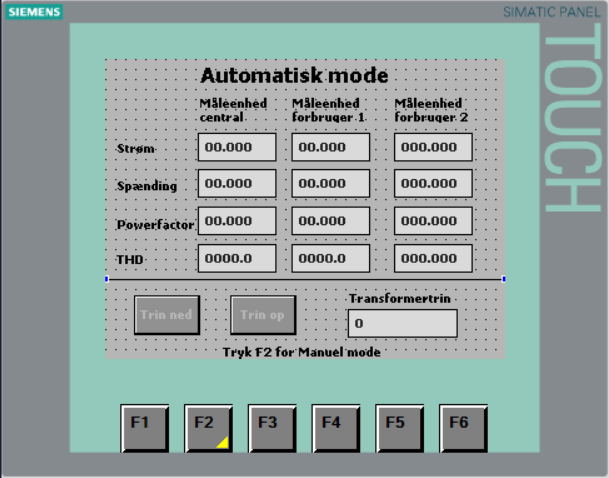
\includegraphics[width=0.7\textwidth]{Figure/HMIAutomatiskModeDesign}
	\caption{Screenshot af HMI i automatisk mode}
	\label{fig:HMIAutomatiskModeDesign}
\end{figure}

For at skifte til manuel mode trykkes på knappen F2. Knappen er valgt for at det er tydeligt at et tryk ville indebære en stor ændring i programmet. Det er også skrevet på selve skærmen for at gøre en bruger opmærksom på tilstandsskiftet. Måden skiftet er programmeret er gennem eventet Press Key og funktionen ActivateScreen, som kan ses på figur \ref{fig:ActivateScreen}.

\begin{figure}[H] % (alternativt [H])
	\centering
	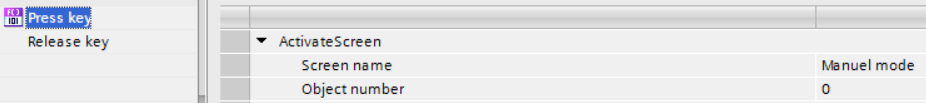
\includegraphics[width=0.8\textwidth]{Figure/ActivateScreen}
	\caption{Aktiver manuel mode skærmen}
	\label{fig:ActivateScreen}
\end{figure}

Måleværdierne er koblet med de word arrays DataCentralEnhed og DataDecentralEnhed tidligere omtalt i afsnit \ref{sec:TCPkommunikation}. Dette sker gennnem opsætning af Inoutblokkene. Et eksempel kan ses på figur \ref{fig:OutputblokMaelingStroemCentral} for strømmen ved den centrale måleenhed, hvor det tilknyttede PLC tag er DataCentralEnhed[0]. Plads 0 er altid strømmen, ligegyldigt hvilket array der tales om. Plads 1 er spændingen, plads 2 er powerfactor og plads 3 er THD. Mode er sat til output, dvs. at man ikke kan ændre værdien gennem skærmen. Formatet er et decimaltal med to decimaler før punktummet og tre decimaler efter punktummet.
Værdien blokkene er tilknyttet er for strøm og spænding i milliammpere og millivolt, derfor er kommaet flyttede tre pladser frem, så værdierne der vises er i ampere og volt.


Det forventes ikke at systemet under normale omstændigheder viser tal større end 7 volt, men to decimaler før kommaet er blevet valgt for at systemet kan vise selv meget store målinger, grundet eventuelle fejl på distributionslinjen. Powerfactor er i transmissionen af data også blevet gjort 1000 gange større og derfor flyttes punktummet også tre pladser her. THD er før transmissionen et decimaltal, som er forstørret 1000 gange, så her er punktummet flyttet en plads for at det kan vises i procent for brugeren.

\begin{figure}[H] % (alternativt [H])
	\centering
	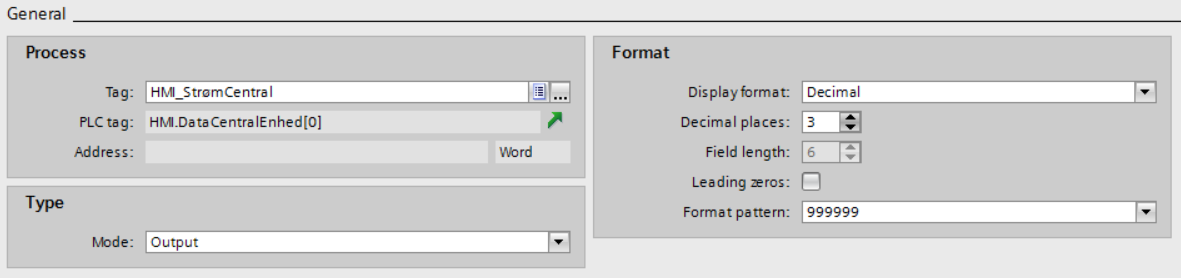
\includegraphics[width=1\textwidth]{Figure/OutputblokMaelingStroemCentral}
	\caption{Inoutblok for strømmåling ved central Måleenhed}
	\label{fig:OutputblokMaelingStroemCentral}
\end{figure}

Til visning af transformertrin er også valgt en Inoutblok, i mode output og tilknyttet PLC tagget Trin brugt i FB'en Trinskifter. Trykknapperne Trin ned og Trin op er gråskalerede for at vise at de ikke er anvendelige i dette mode.

\subsection{Manuel mode}

Gennemgående er den samme model brugt til Manuel mode, men der er to forskelle. Den første er at for at skifte til automatisk mode skal bruges knappen F1, hvilket også er tydeliggjort ved en tekst nederst på skærmen.


Den anden er at knapperne Trin ned og Trin Op nu er aktive og kan bruges. Valget af sort tekst på hvid baggrund gør det nemt for en bruger at spotte at knapperne kan bruges. Figur \ref{fig:HMIManuelModeDesign} viser Manuel mode.

\begin{figure}[H] % (alternativt [H])
	\centering
	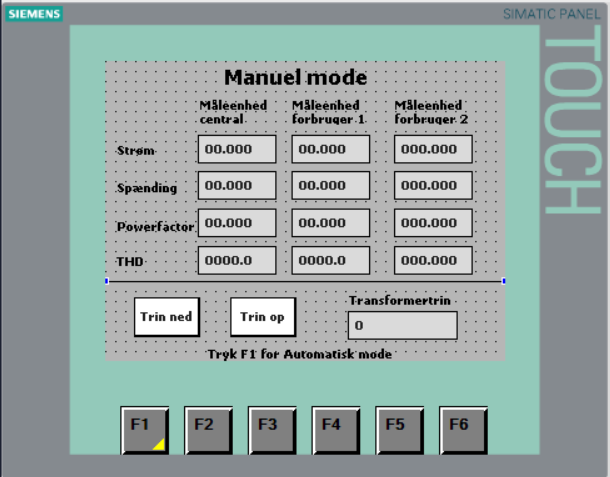
\includegraphics[width=0.5\textwidth]{Figure/HMIManuelModeDesign}
	\caption{Screenshot af HMI i manuel mode}
	\label{fig:HMIManuelModeDesign}
\end{figure}

Knappen er sat til at man ved et tryk sætter et bit, her er det tagget HMI\_KnapOp, der er tilknyttet PLC tagget KnapOp som anvendes i FB'en Trinskifter. Se figur \ref{fig:HMITrinOp}. Når knappen slippes er funktionen ResetBit anvendt, som resetter HMI\_KnapOp. Trin ned har samme funktionalitet, her er det bare HMI\_KnapNed, der anvendes, som er tilknyttet KnapNed i FB'en Trinskifter.

\begin{figure}[H] % (alternativt [H])
	\centering
	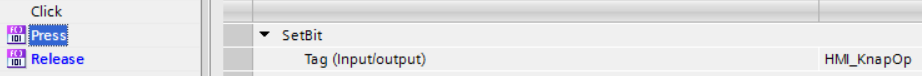
\includegraphics[width=0.8\textwidth]{Figure/HMITrinOp}
	\caption{Funktionalitet bag Trin op knappen}
	\label{fig:HMITrinOp}
\end{figure}

Ved tryk på knapperne F1 og F2 aktiveres skærmen for, henholdsvis automatisk og manuel mode, men dette sætter ikke programmet i de tilsvarende tilstand. Det sker i øjeblikket den pågældende skærm bliver loaded. Tilstanden styres af et bit der har HMI tagget HMI\_ManuelMode og PLC tagget ManuelMode. På figur \ref{fig:LoadManuelModeSkaerm} kan man se at når manuel mode skærmen loades kaldes SetBit funktionen. For automatisk mode skærmen kaldes funktionen ResetBit på samme bit.

\begin{figure}[H] % (alternativt [H])
	\centering
	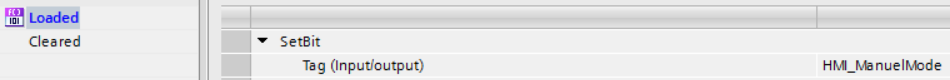
\includegraphics[width=0.8\textwidth]{Figure/LoadManuelModeSkaerm}
	\caption{Aktivering af manuel mode når manuel mode skærmen loades}
	\label{fig:LoadManuelModeSkaerm}
\end{figure}

Generelt er skærmene udviklet med henblik på at det er nemt få overblik over dem og at de er nemme at forstå. Der er valgt at ligge vægt på få muligheder, fordi det er et system som der skal sikres mod forkert brug, da det kan få store konsekvenser.
% !TEX root = ../../prj4projektdokumentation.tex

\section{Kommunikationsmodul}

Kommunikationsmodulets egenskaber er at indsamle data fra måleenheder og sende dem videre til kontrolmodulet. Kommunikations modulet består af en Arduino Mega2560 med et tilknyttet Ethernet Shield R3. Dette shield er designet med udgangspunkt i W5100-microchippen, der er en standard ethernet controller chip. Dette ethernet shield bliver opsat fra Arduinoen igennem en SPI forbindelse, der oprettes i Arduino koden. 

Kommunikationsmodulet efterspørger måledata fra måleenheden over en UART forbindelse. Da der kan kobles mange enheder op på samme UART linje, vil kommunikationsmodulet være i stand til at hente information fra så mange måleenheder som ønskes. Hvis der kobles flere måleenheder på samme UART linje kræver det blot en lille ændring i protokollen, således der ikke opstår situationer hvor 2 enheder sender data retur samtidig. 


Herunder ses et eksempel af koden, hvor kommunikationsmodulet modtager data fra måleenhederne. For at få en bedre opløsning i målingerne bliver der sendt 16 bit, som er realiseret ved at dele 16bit op i to 8bits: 

\lstset{caption={Modtagelse},label={ModtagelsesKode}}
\begin{lstlisting} % Start your code-block
  Serial1.write('A');
  
  while(read1!=1);
  read1 = 0;
  
  MCStrom = Serial1.read();
  delay(3);
  MCStrom1 = Serial1.read();
\end{lstlisting}


For hver måledata er der oprettet 2 integers, der skrives til individuelt. Dette ses med MCStrom og MCStrom1, der tilsammen giver måleenhedens strømværdi i milliampere. 
Den variable read1, der ses i kodeeksemplet \ref{ModtagelsesKode} er interruptstyret. Interruptet er benyttet for at vente på måleenheden får samplet en hel periode. Interruptet er implementeret på følgende måde i Arduinokoden: 

\lstset{caption={Interrupt},label={InterruptKode}}
\begin{lstlisting} % Start your code-block

// Skrevet i den globale del af koden:

int receive()
{
	read1 = 1;
}

// Skrevet i setup-delen:

  attachInterrupt(digitalPinToInterrupt(19),receive, RISING);

\end{lstlisting}


Funktionen attachInterrupt() er en allerede implementeret funktion i Arduino udviklingsværktøjet. Funktionen skal have 3 parametre, hvor den første er lidt speciel, da den skal hedde digitalPinToInterrupt(pin), hvor pin er nummeret på arduinopinen der skal interruptes. Den anden parameter er navnet på Interrupt Service Routinen der skal køres når der fås et interrupt på pinen. Den sidste parameter bestemmer om interruptet skal triggeres på en lav værdi, et skift i tilstand, en rising edge eller falling edge. Der er i dette tilfælde valgt et interrupte på rising edge, da det er en UART-modtagelse der skal interruptes på. 

Opsætningen af ethernet på Arduinoen: 


\lstset{caption={Ethernet},label={EthernetKode}}
\begin{lstlisting} % Start your code-block


// Skrevet i den globale del af koden:
#include <SPI.h>
#include <Ethernet.h>

byte mac[] = {0x90, 0xA2, 0xDA, 0x0F, 0x1B, 0x82};   // MAC Address
byte ip[] = {192, 168, 0, 129};                // Network Address


EthernetServer server = EthernetServer(27015);


// Skrevet i setup delen af koden:
      Ethernet.begin(mac,ip);
      server.begin();



\end{lstlisting}

% !TEX root =../prj4projektrapport.tex

\section{Modultest}


% !TEX root = ../../prj4projektdokumentation.tex

\chapter{Integrationstest}

\section{Integrationstest mellem Måleenhed og Styringsenhed}

I dette afsnit testes kommunikationen mellem Måleenhed og Brugergrænsefladen. Der vil blive testet af de rigtig tal vises på skærmen, hastigheden mellem opdatering af visninger samt pålideligheden af dokumentationen. Testopstilling kan ses på figur \ref{fig:opstilling1}.

\begin{figure}[htbp] % (alternativt [H])
	\centering
	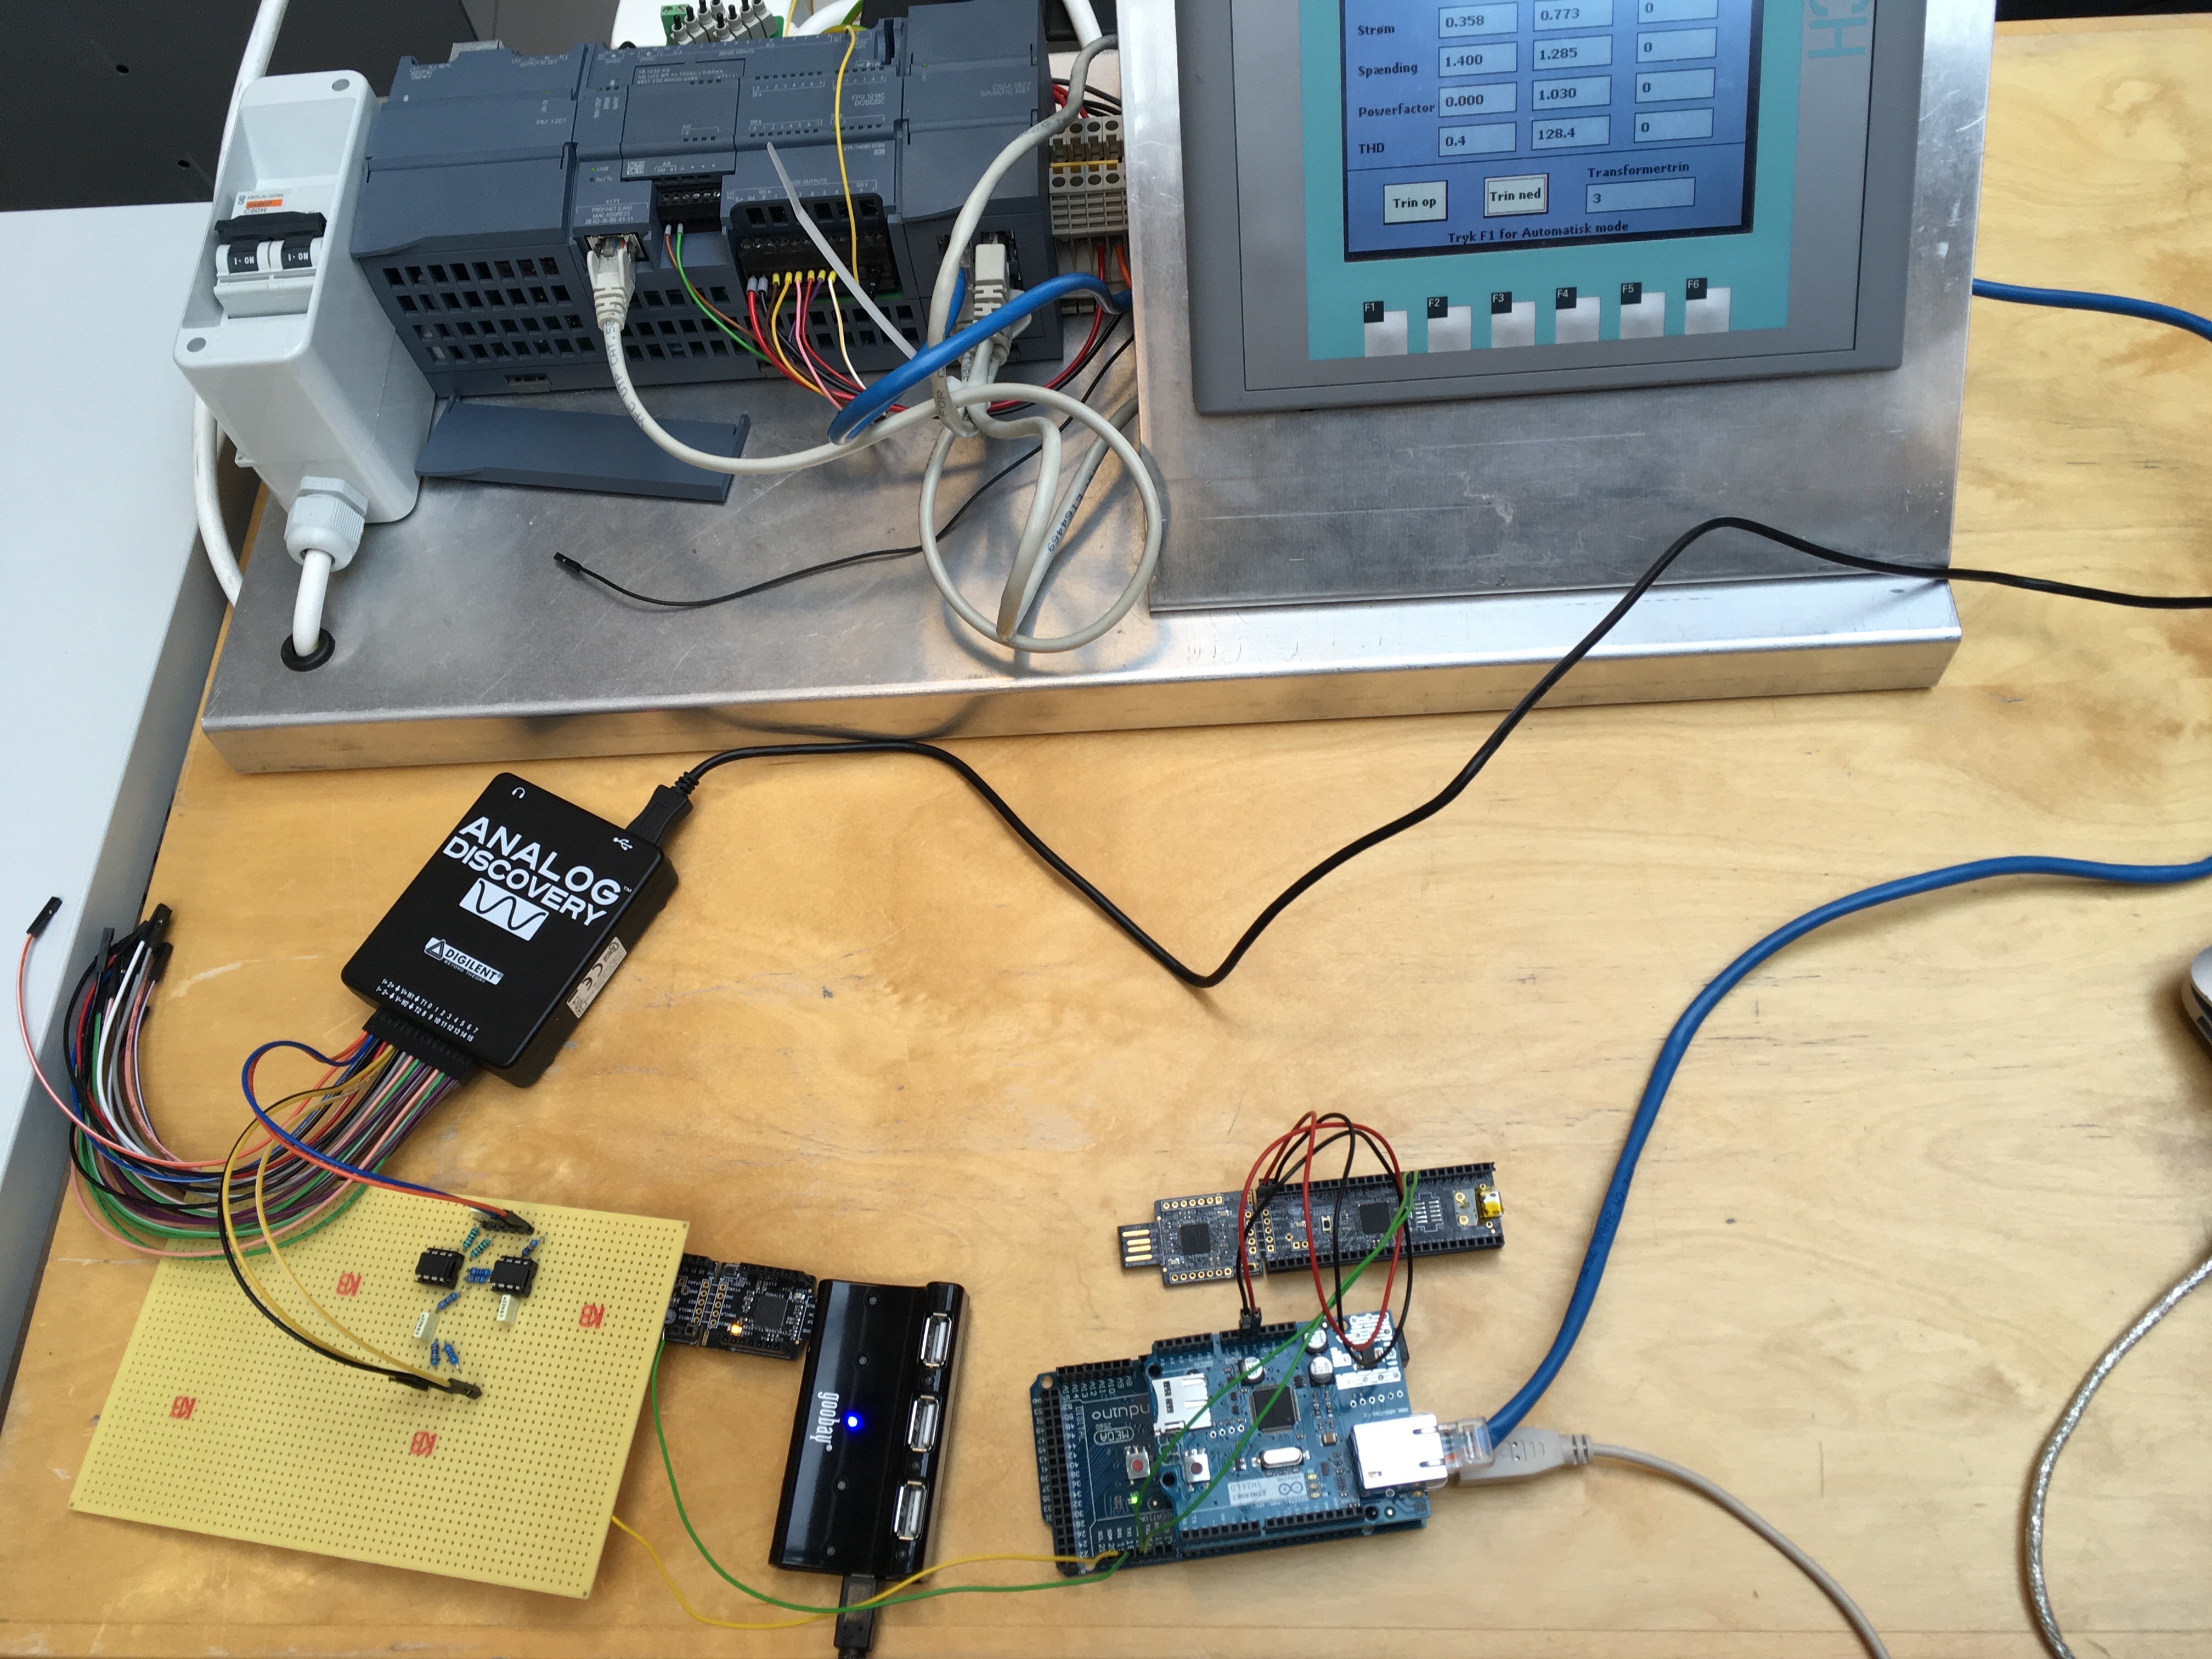
\includegraphics[width=0.7\textwidth]{Test/Opstilling1}
	\caption{Testopstilling af integrationstest mellem Måleenhed og Styringsenhed}
	\label{fig:opstilling1}
\end{figure}

Til testen skal der bruges:
\begin{itemize}
	\item 1 stk PSOC
	\item 1 stk Arduino med ethernet shield
	\item 1 stk PLC med hmi skærm
	\item Ledning fra PSOC's UART til Arduino
	\item Ethernet ledning fra ethernet shield til PLC
	\item Analog Discovery
\end{itemize}

\begin{table}
	\begin{tabular}{ | m{0.2\textwidth} | m{0.8\textwidth}|} 
		\hline
		\textbf{Test}					&Brugergrænsefladen modtager korrekte tal \\ \hline
		\textbf{Testbeskrivelse}		&Der testes at de værdier, der kommer ind på Måleenheden er ens med værdierne der vises på brugergrænsefladen. \\ \hline
		\textbf{Input}					&Analog Discovery anvendes til at lave 4VPP sinus på spænding indgang, 1VPP sinus på strøm indgang, 3,3ms forskydning \\ \hline
		\textbf{Forventet output}		&1,414V spænding, 0,354A strøm, 0,509 PF se figur \ref{fig:PFtest1}, 0 THD \\ \hline
		\textbf{Resultat}				&1,404V spænding, 0,359A strøm, 0,491, 0,2 THD,  se figur \ref*{fig:visningtest1} for resultat af skærm  \\ \hline
	\end{tabular}
	\caption{Integrationstest 1} 
\label{tab:int test 1} 
\end{table}

\begin{figure}[H] % (alternativt [H])
	\centering
	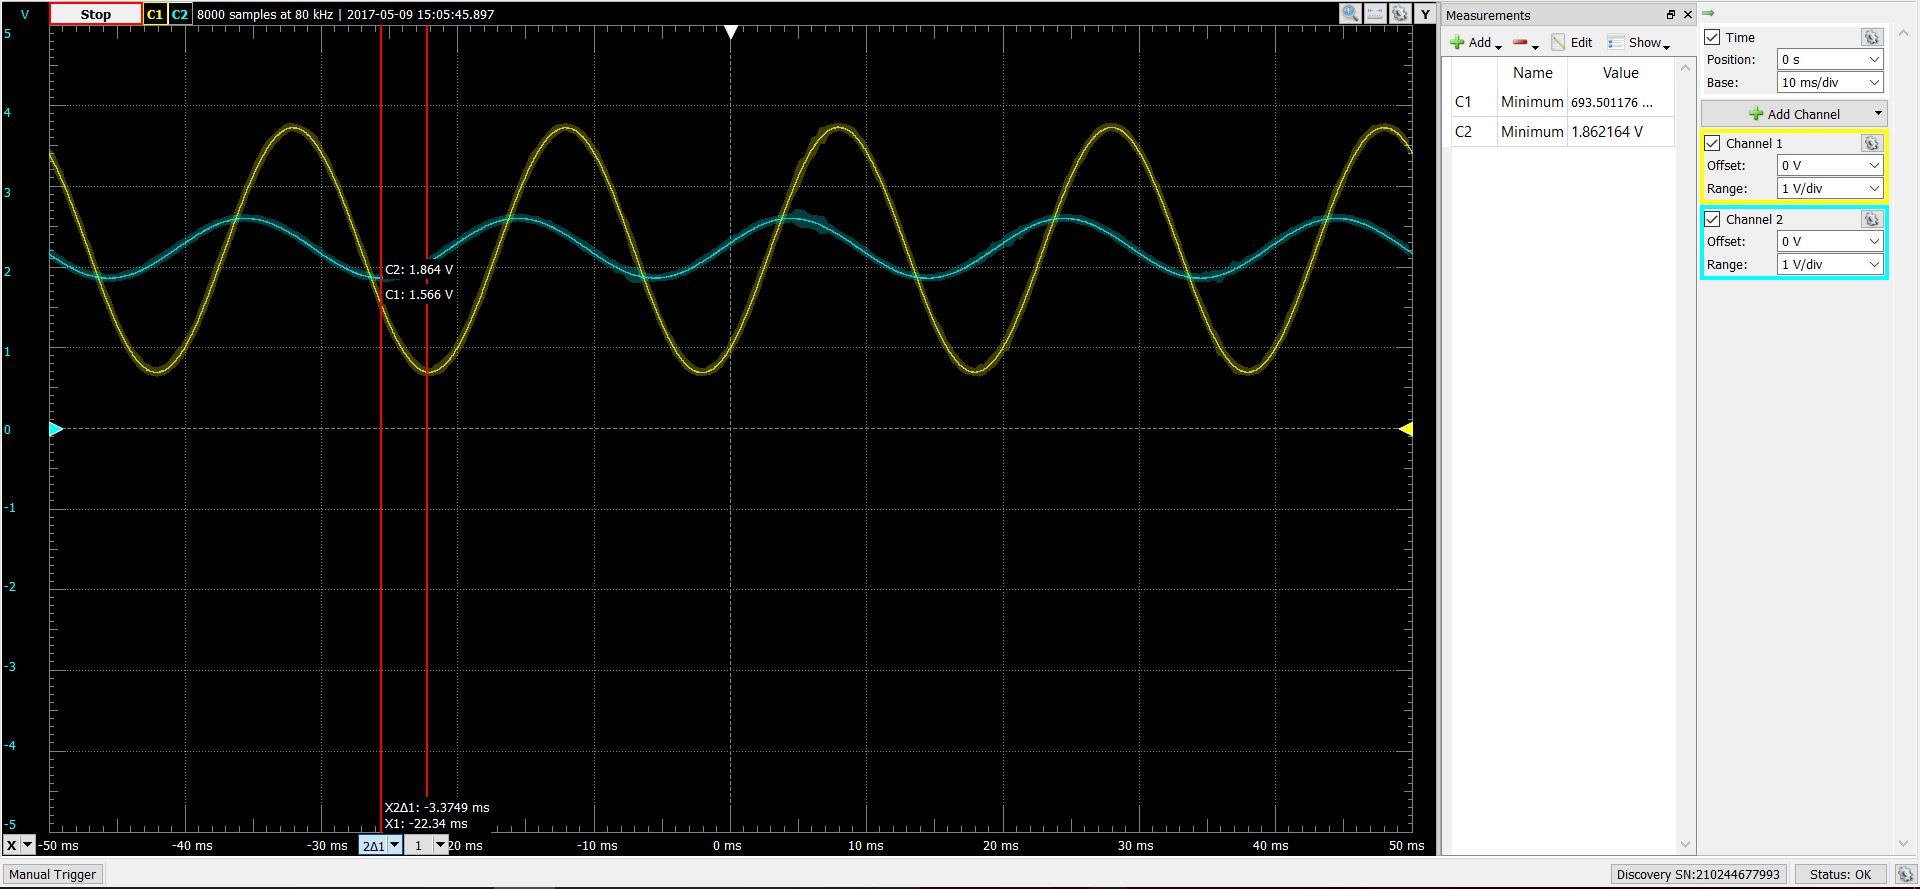
\includegraphics[width=0.7\textwidth]{Test/PFTest1}
	\caption{Visning af 3,3ms forsinkelse mellem strøm og spænding}
	\label{fig:PFtest1}
\end{figure}

\begin{figure}[H] % (alternativt [H])
	\centering
	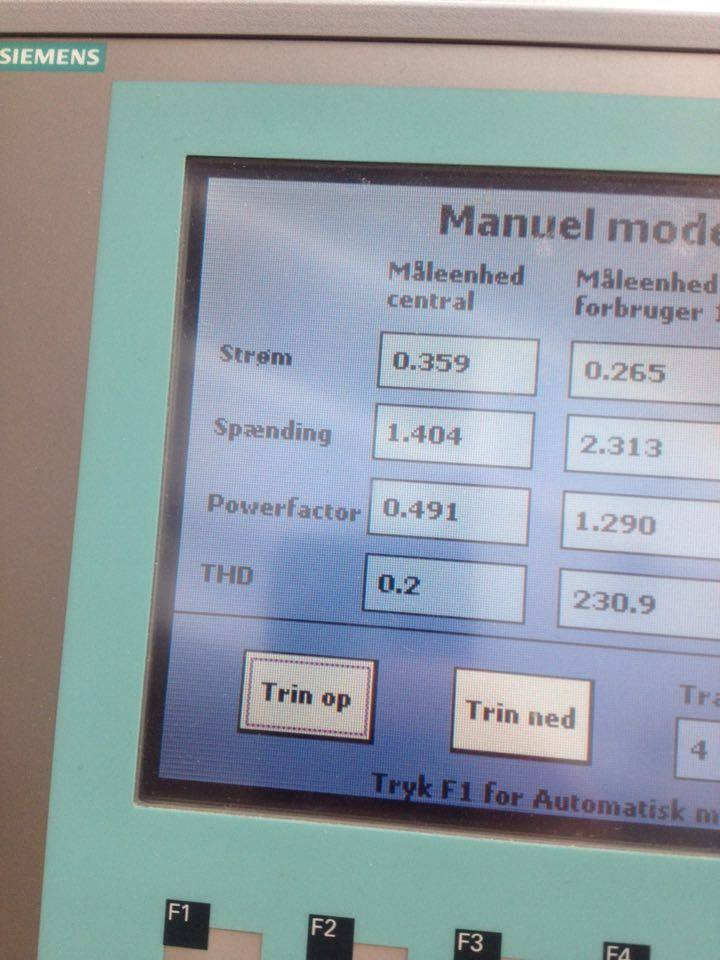
\includegraphics[width=0.5\textwidth]{Test/Visningstest1}
	\caption{Resultatet af visning på brugergrænseflade}
	\label{fig:visningtest1}
\end{figure}


\begin{table}
	\begin{tabular}{ | m{0.2\textwidth} | m{0.8\textwidth}|} 
		\hline
		\textbf{Test}					&Forsinkelse på brugergrænsefladen \\ \hline
		\textbf{Testbeskrivelse}		&Tiden der går fra mellem ændringer på skærmen \\ \hline
		\textbf{Input}					&4VPP \\ \hline
		\textbf{Forventet output}		&At der maks. går 2,5 sekund, pga intern delay i PLC og kommunikation \\ \hline
		\textbf{Resultat}				&Der er målt 5 gange: 2,01s 2,00s 1,99s 2,00s 1,95s, der alle har vist sig at være inden for kravet.   \\ \hline
	\end{tabular}
	\caption{Integrationstest 2} 
\label{tab:int test 2} 
\end{table}


\begin{table}
	\begin{tabular}{ | m{0.2\textwidth} | m{0.8\textwidth}|} 
		\hline
		\textbf{Test}					&Kommunikations pålidelighed \\ \hline
		\textbf{Testbeskrivelse}		&Der observeres på brugergrænsefladen i 1 min og tælles uregelmæssigheder \\ \hline
		\textbf{Input}					&4VPP sinus på spænding indgang, 1VPP sinus på strøm indgang\\ \hline
		\textbf{Forventet output}		&5\% fejl ud af 120 inputs \\ \hline
		\textbf{Resultat}				&5 fejl dvs. 4.17\%  \\ \hline
	\end{tabular}
	\caption{Integrationstest 3} 
\label{tab:int test 3} 
\end{table}

% !TEX root = ../../prj4projektdokumentation.tex

\section{Samlet integrationstest}
Denne test indeholder alle de enkelte moduler, som systemet består af, herunder Brugergrænseflade, Måleenhed, Styringsenhed og Trinskifter. 

I dette afsnit testes at udregninger for hvordan nettet opfører sig stemmer overens med det, der måles med Måleenheden, og det der vises på brugergrænsefladen.
Testene laves ved at måle på nettet med Måleenheden, som er forbundet til brugergrænsefladen, så resultaterne for målinger kan aflæses på skærmen. Værdierne sammenholdes med resultaterne fra simulering og beregning. 



\begin{table}[H]
	\begin{tabular}{ | m{0.2\textwidth} | m{0.8\textwidth}|} 
		\hline
		\textbf{Test}					&Udregning og simulering passer med systemets værdier. \\ \hline
		\textbf{Testbeskrivelse}		&Der testes ved at forsyne nettet med trinskifteren og derefter måle spænding, strøm og Pf med Måleenheden ved en forbruger \\ \hline
		\textbf{Input}					&4Vrms fra trinskifter, der tilsluttes 54$\Omega$ belastning efter distributionslinjen \\ \hline
		\textbf{Forventet output}		&At resultaterne i tabel \ref{tab:intTest2} stemmer overens \\ \hline
		\textbf{Resultat}				&Se tabel \ref{tab:intTest2} \\ \hline
	\end{tabular}
	\caption{Integrationstest 4}
\label{tab:intTest4}
\end{table}


\begin{table}[H]
	\begin{tabular}{ | m{0.2\textwidth} | m{0.2\textwidth} | m{0.2\textwidth} | m{0.2\textwidth}|}  
		\hline
		\textbf{Test}			& \textbf{Spænding} & \textbf{Strøm}  	& \textbf{PF}			\\ \hline
		\textbf{Simulering}		&3,580V					&0,066A				  	&0,997 					\\ \hline
		\textbf{Beregnet}		&3,600V 					&0,066A					&0,996					\\ \hline
		\textbf{Målt}			&3,379V					&0,058A					&0,999				\\ \hline
	\end{tabular}
	\caption{Resultat af Integrationstest 4}
	\label{tab:intTest4result}
\end{table}

\begin{figure}[H] 
	\centering
	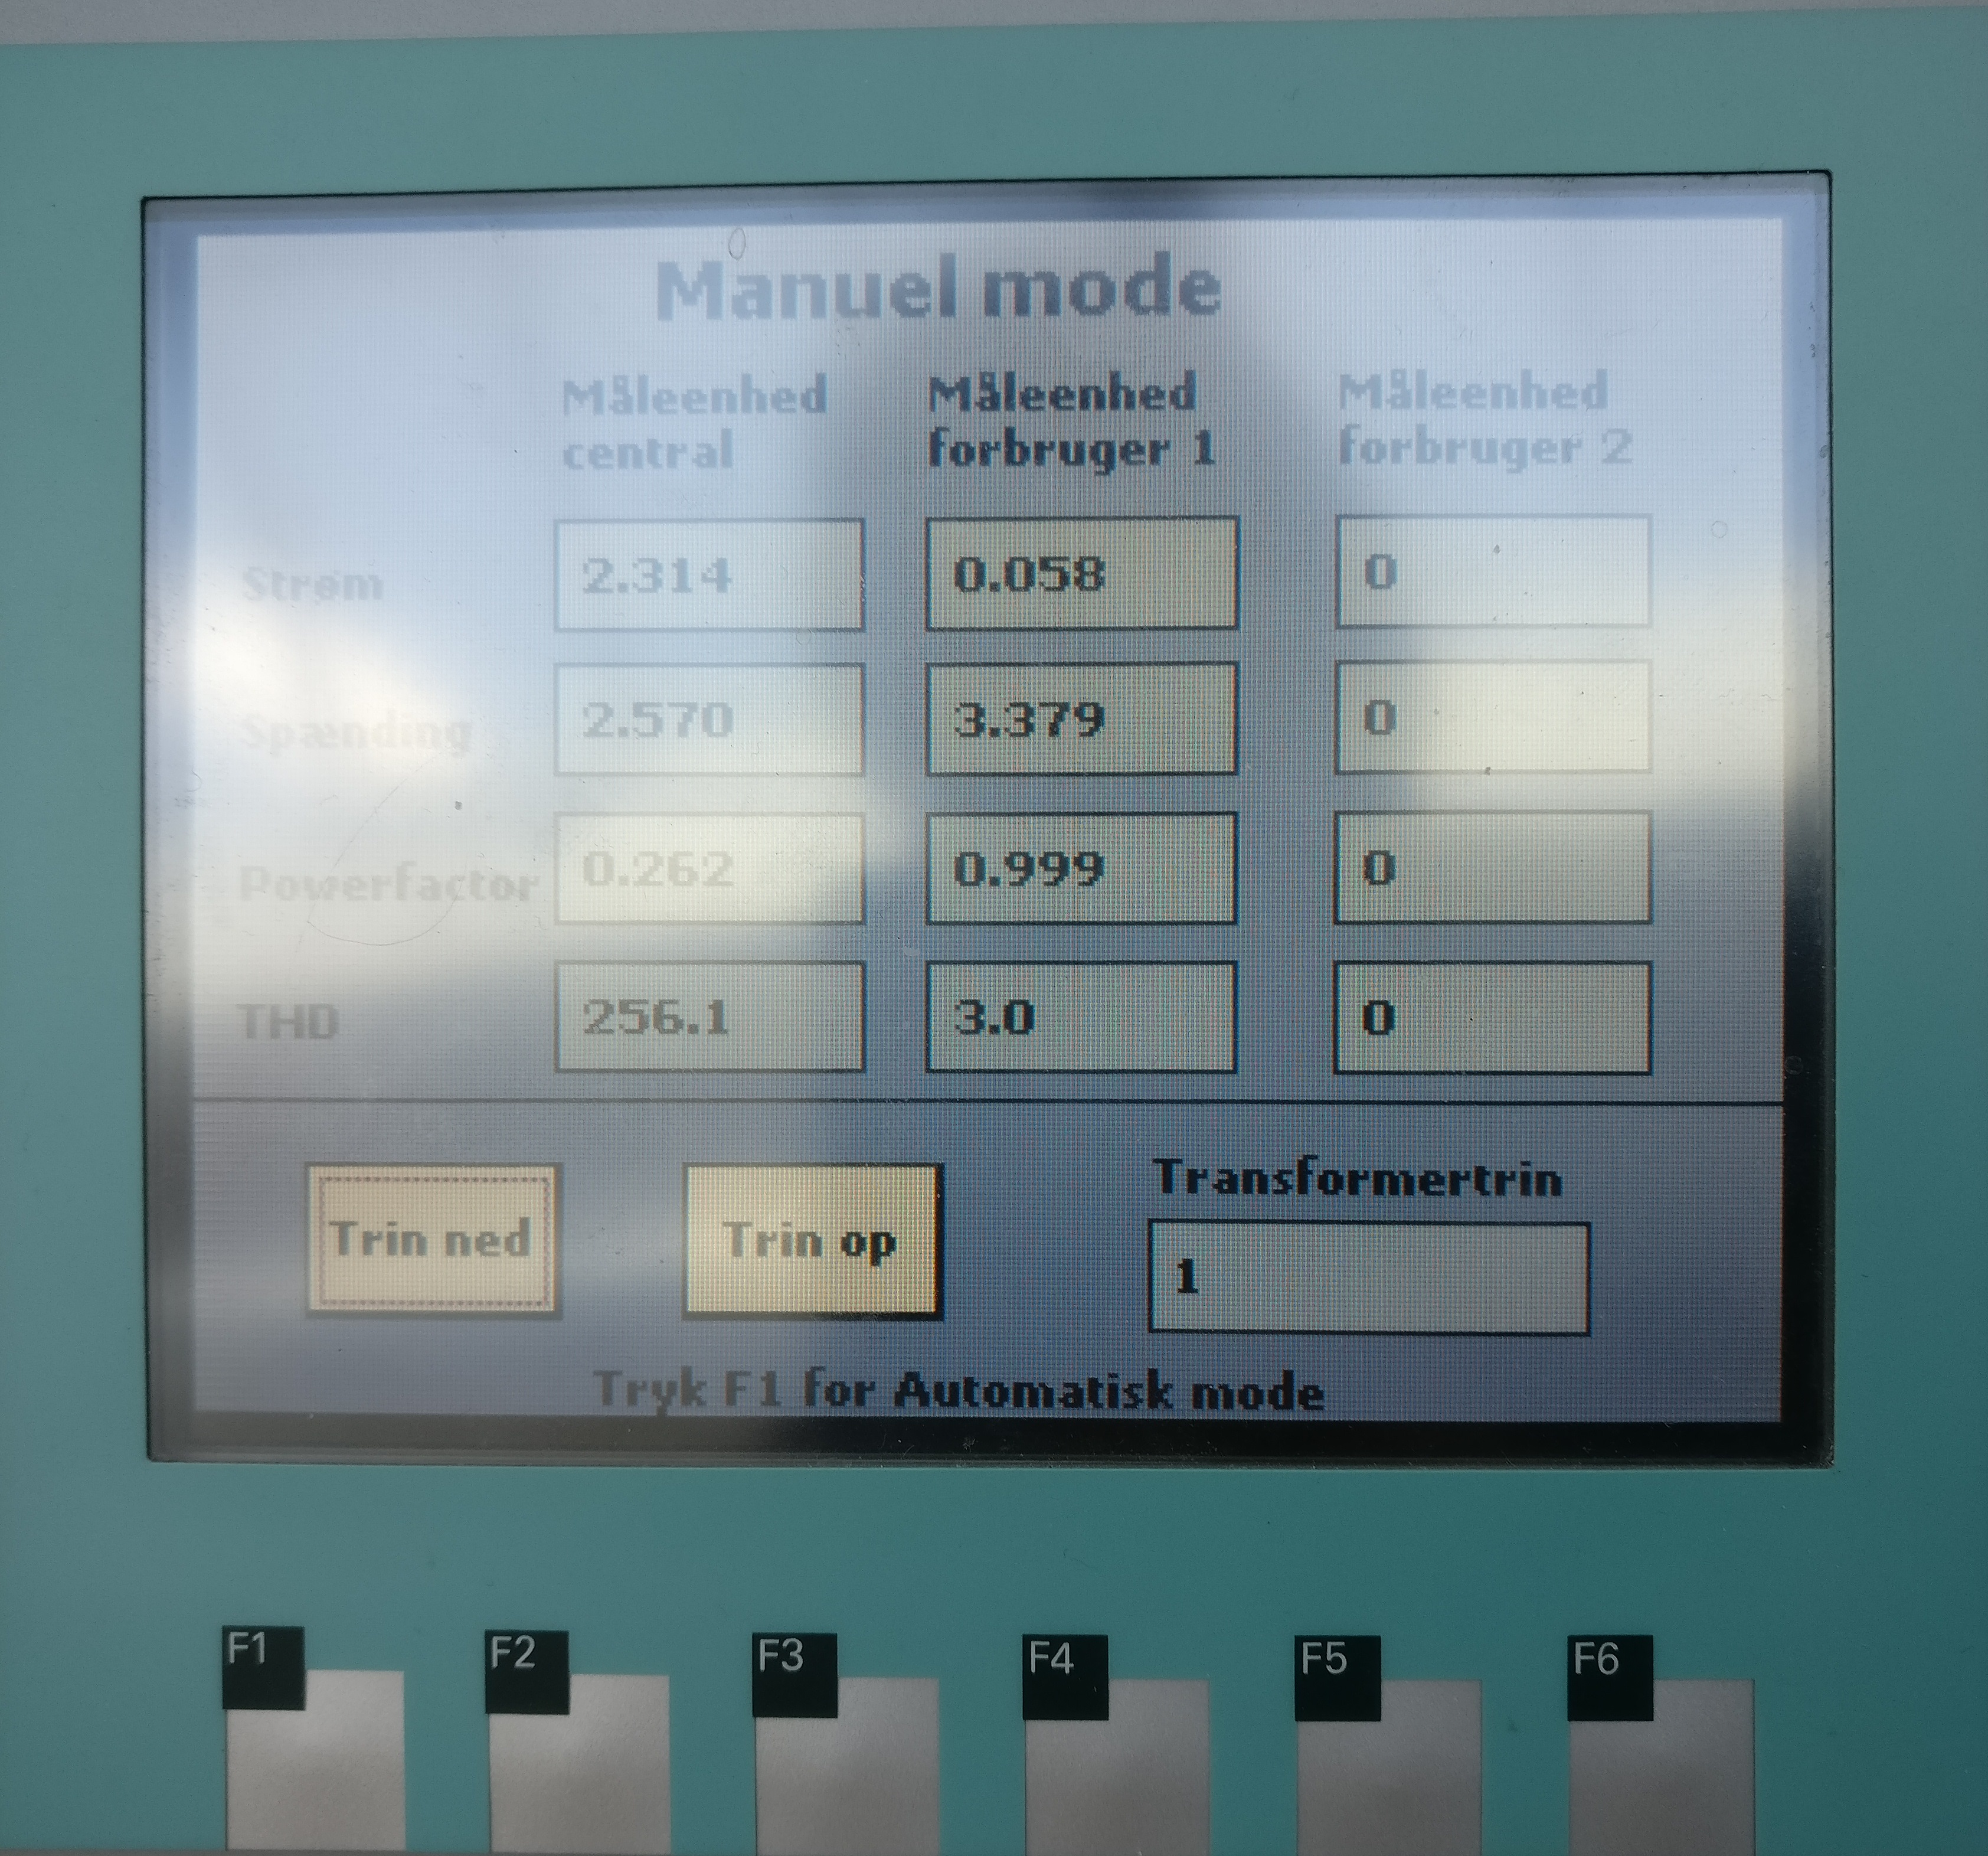
\includegraphics[width=0.7\textwidth]{Figure/INT4}
	\caption{Resultat af integrationstest 4, målteværdier.}
	\label{fig:INT4Mal}
\end{figure}



Opstillingen til den samlede integrationstest kan ses på figur \ref{fig:Opstilling1} og \ref{fig:Opstilling2}

\begin{figure}[H] 
	\centering
	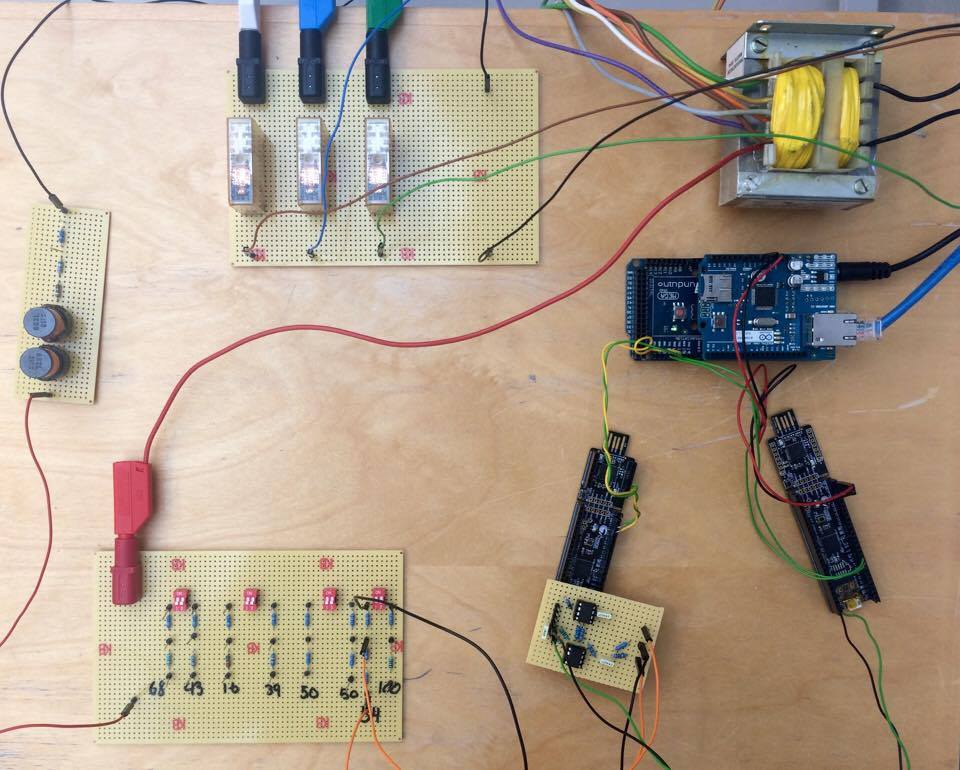
\includegraphics[width=0.7\textwidth]{Figure/Opstillingudenplc}
	\caption{Opstilling af samlet system uden PLC}
	\label{fig:Opstilling1}
\end{figure}

\begin{figure}[H] 
	\centering
	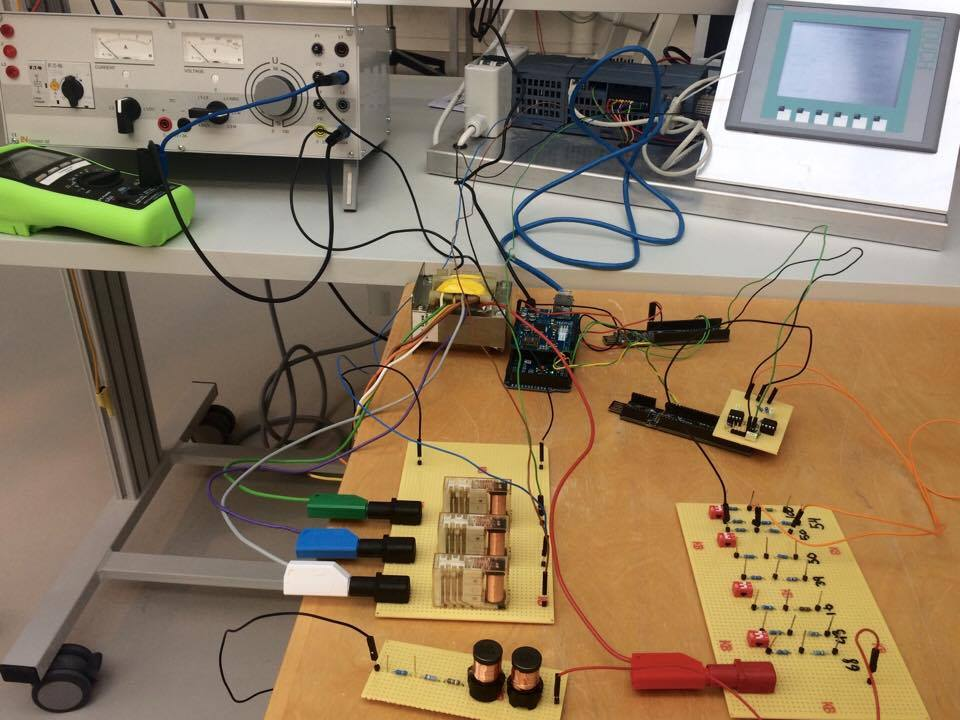
\includegraphics[width=0.7\textwidth]{Figure/Opstillingmedplc}
	\caption{Opstilling af samlet system med PLC}
	\label{fig:Opstilling2}
\end{figure}
\chapter{Accepttest}

% !TEX root = ../../prj4projektdokumentation.tex

\section{Funktionelle Krav}
%usecase 1
\begin{table}[htbp]
	\centering
	\begin{tabular}{|p{2cm}|p{3cm}|p{4cm}|p{4.5cm}|p{1cm}|}
		\hline
		\textbf{UC1} & \textbf{Handling} & \textbf{Forventet resultat} & \textbf{Resultat} &\textbf{OK} \\\hline
		Start manuel styring & Bruger vælger Manuel Mode & På skærmen vises Manuel Mode med mulighed for valg af trin & Skærmen viser Manuel Mode & \checkmark \\\hline
		
		
	\end{tabular}
	
	
\end{table}

%usecase2
\begin{table}[htbp]
	\centering
	\begin{tabular}{|p{2cm}|p{3cm}|p{4cm}|p{4.5cm}|p{1cm}|}
		\hline
		\textbf{UC2} & \textbf{Handling} & \textbf{Forventet resultat} & \textbf{Resultat} &\textbf{OK} \\\hline
		Stop manuel styring & Bruger vælger Automatisk Mode & Skærmen viser Automatisk Mode, hvor trinknapperne er deaktiverede & Der vises Automatisk Mode & \checkmark \\\hline
		
		
	\end{tabular}
\end{table}

% usecase3a
\begin{table}[htbp]
	\centering
	\begin{tabular}{|p{2cm}|p{3cm}|p{4cm}|p{4.5cm}|p{1cm}|}
		\hline
		\textbf{UC3a} & \textbf{Handling} & \textbf{Forventet resultat} & \textbf{Resultat} &\textbf{OK} \\\hline
		Skift trin op & Systemet er i Manuel Mode. Bruger vælger Trin Op på skærmen & Systemet skifter trin op på transformeren og skærmen opdateres med nye værdier. & Transformeren skifter trin efter 2s. Derefter opdateres spænding, strøm, pf og THD på skærmen inden 2s.  & \checkmark \\\hline
		
		
	\end{tabular}
\end{table}

%usecase3b
\begin{table}[H]
	\centering
	\begin{tabular}{|p{2cm}|p{3cm}|p{4cm}|p{4.5cm}|p{1cm}|}
		\hline
		\textbf{UC3b} & \textbf{Handling} & \textbf{Forventet resultat} & \textbf{Resultat} &\textbf{OK} \\\hline
		Skift trin ned & Systemet er i Manuel Mode. Bruger vælger Trin Ned på skærmen & Systemet skifter trin ned på transformeren og skærmen opdateres med nye værdier. & Transformeren skifter trin efter 2s. Derefter opdateres spænding, strøm, pf og THD på skærmen inden 2s.  & \checkmark \\\hline
		
		
	\end{tabular}
	
	
\end{table}

\section{Ikke funktionelle krav}
% for spændingsregulator
\begin{table}[H]
	\centering
	\begin{tabular}{|p{4cm}|p{3cm}|p{3cm}|p{3cm}|p{1cm}|}
		\hline
		\textbf{Trintransformer} & \textbf{Handling} & \textbf{Forventet resultat} & \textbf{Resultat} &\textbf{OK} \\\hline
		Nominel spænding på primærsiden er 24VAC & Spændingen på primærsiden måles. & Den målte værdi er 24VAC. & Der måles 23.88 VAC & \checkmark \\\hline
		Nominel spænding på sekundær side er 4, 5 eller 6 VAC afhængig af trin & Spændingen på sekundærsiden måles for hhv. trin 4, 5 og 6. & Den målte værdi er 4, 5 eller 6 VAC alt efter valgt trin. & Der måles hhv. 4, 5 og 6 VAC & \checkmark \\\hline
		Skal minimum kunne levere 500mA	. & Strømmen på sekundærsiden måles. & Transformeren kan levere over 500mA & xx  & xx \\\hline
	\end{tabular}
	
\end{table}

% for belastning
\begin{table}[H]
	\centering
	\begin{tabular}{|p{4cm}|p{3cm}|p{3cm}|p{3cm}|p{1cm}|}
		\hline
		\textbf{Belastning} & \textbf{Handling} & \textbf{Forventet resultat} & \textbf{Resultat} &\textbf{OK} \\\hline
		Modstandsværdi på 54$\Omega$ giver spændingsfald på 10\%, når spændingen fra regulatoren er 4V. & Den givne modstand indsættes som belastning, og spændingen herover måles. & Spændingen over belastningen måles til 3,6V. & xx & xx \\\hline	
	\end{tabular}
	
	
\end{table}

% for måleenhed
%\begin{table}[htbp]
%	\centering
\begin{longtable}{|p{4cm}|p{3cm}|p{3cm}|p{3cm}|p{1cm}|}
	\hline
	\textbf{Måleenhed} & \textbf{Handling} & \textbf{Forventet resultat} & \textbf{Resultat} &\textbf{OK} \\\hline
	Måle spændingen ved trinskifteren og forbrugerne mellem 0 og 8 Vrms & Måleenheden testes med spændinger fra 0 til 8Vrms, i intervaller af 500mV. & Korrekt spændingsmåling i hele intervallet. & Korrekte spændingsmålinger i hele intervallet & \checkmark\\\hline
	Måle spændingen med en præcision på $\pm$ 5\%& Måleenheden påtrykkes en spænding på 3,5Vrms. Der laves herefter ti målinger& Gennemsnits afvigelsen forventes at være under $\pm$5\%.& Afvigelsen er fundet til 1,6\%. &\checkmark\\\hline
	Måle strømmen ved trinskifteren og forbrugerne mellem 0 og 500mA& Måleenheden testes med strømme fra 0 til 500mA i intervaller af 50mA&Korrekt strømmåling i hele intervallet.&Korrekt strømmåling i hele intervallet&\checkmark\\\hline
	Måle strømmen med en præcision på $\pm$ 5\%&Måleenheden påtrykkes en spænding på 300mVrms (Svarende til 300mA), der laves herefter ti målinger&Gennemsnits afvigelsen forventes at være under $\pm$5\%&Afvigelsen er fundet til 0,8\%.&\checkmark\\\hline
	Måle og beregne power factor med en præcision på $\pm$ 5$\%$&Måleenheden måler power factor over en belastning på distributionslinjen, der sammenlignes med beregnet power factor&Afvigelsen forventes at være under $\pm$ 5\% &Afvigelsen er fundet til ??&xx\\\hline
	Beregne THD med en præcision på $\pm$ 5$\%$&Måleenheden påtrykkes en firkantsignal med 1V amplituder og 1V offset. Der sammenlignes med beregnet THD for firkantsignal& Afvigelsen forventes at være under $\pm$ 5\%&Afvigelsen er fundet til 0,5\%&\checkmark\\\hline
	
\end{longtable}


%\end{table}
% !TEX root = ../../prj4projektdokumentation.tex
\chapter{Metode}


Til gennemførelse af dette projekt er ASE-modellen blevet anvendt som udgangspunkt. Denne model viser de forskellige faser, projektgruppen skal igennem på vejen mod et endeligt produkt og en veldokumenteret og gennemarbejdet rapport. ASE-modellen ses på figur \ref{fig:Asemodel} Gruppen har desuden anvendt en iterativ og empirisk arbejdsmetode. Der er brugt faglitteratur og teori fra undervisningen til at danne vidensgrundlag for projektet om spændingsregulatoren. Undervejs er der indsamlet nye erfaringer i forbindelse med udviklingen af produktet. 
I udviklingsfasen er der anvendt SysML og UML, der sammen med Use Casene har givet overblik over systemet både grafisk og skriftligt. Dette har dannet grundlag for opbygningen af systemet. 

\begin{figure}[H] 
	\centering
	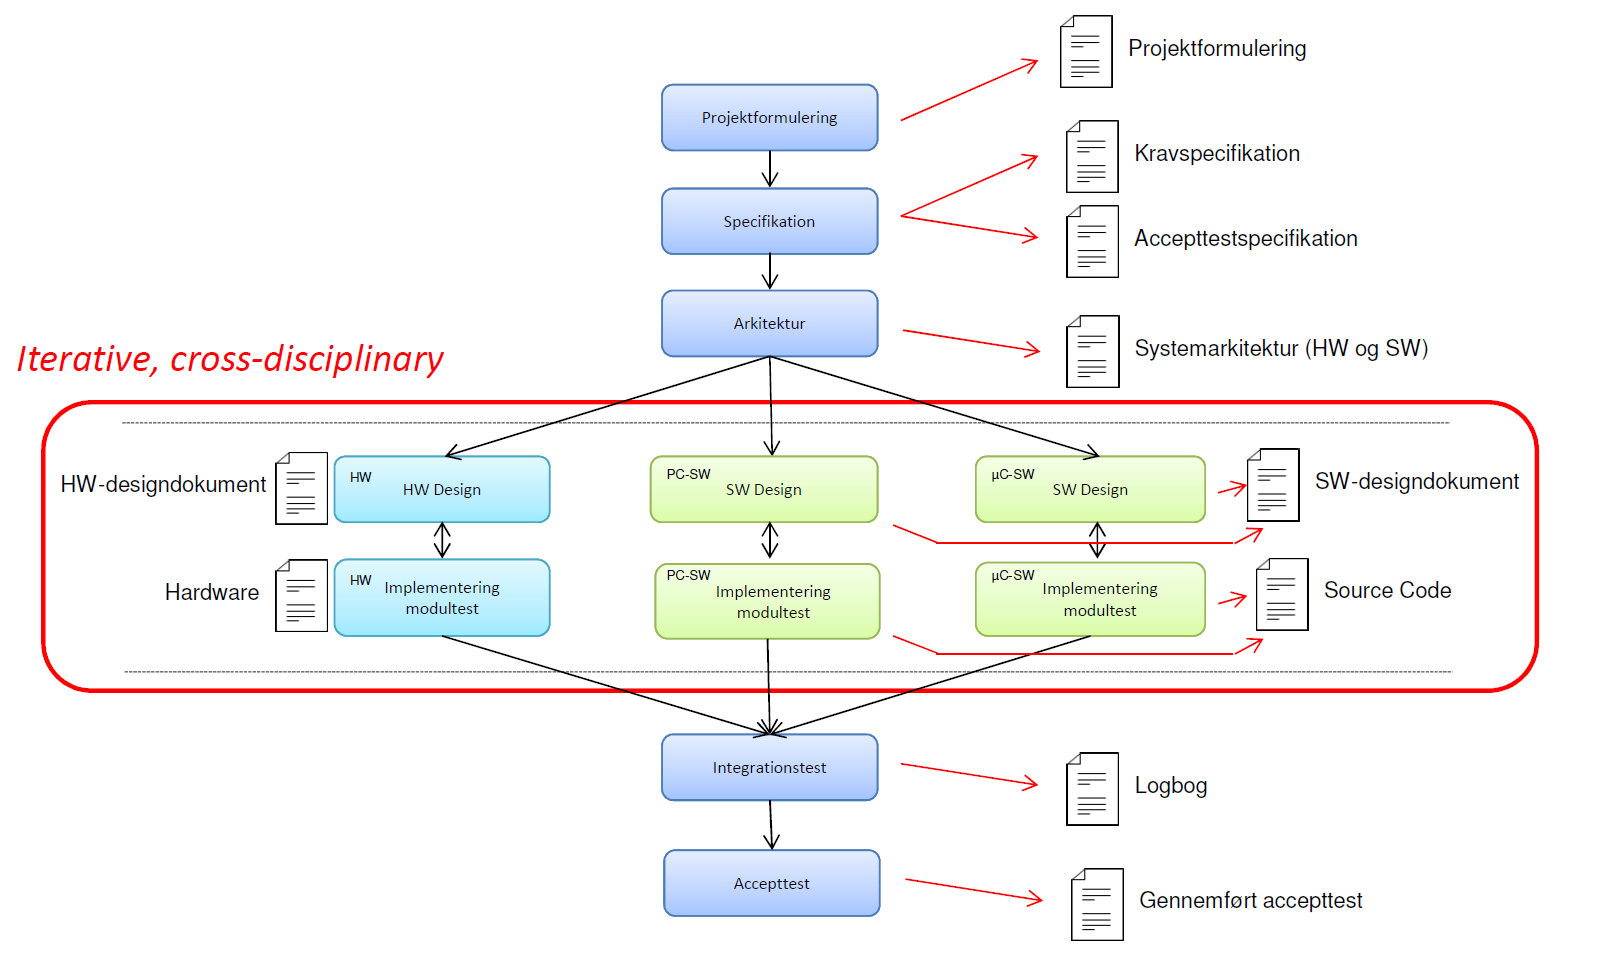
\includegraphics[width=0.7\textwidth]{Figure/Asemodel}
	\caption{Asemodellen}
	\label{fig:Asemodel}
\end{figure}

For at styre og lede projektet har gruppen ladet sig inspirere af Scrum principperne. Fra starten af projektet har gruppen oprettet sprints og defineret dertilhørende opgaver. Gruppen har ikke afholdt daily scrums, men har gennemsnitligt haft 1-2 ugentlige gruppemøder, samt ugentligt vejledermøde. Dette har medført en jævn arbejdsgang og et godt flow i projektet. 
\printbibliography
\end{document}


